\documentclass[12pt]{article}
\usepackage[spanish]{babel}
\usepackage{geometry}
 \geometry{
 a4paper,
 left=25mm,
 right=25mm,
 top=30mm
 }
\usepackage[utf8]{inputenc} 
\usepackage[shortlabels]{enumitem}
\usepackage{hyperref}
\usepackage{wrapfig}
\usepackage[rflt]{floatflt}
\usepackage[pdftex]{graphicx}
\usepackage{fancyhdr}
\usepackage{float}
\usepackage{longtable,multirow,booktabs}
\usepackage{cite}
\usepackage{wrapfig}
\usepackage{multicol}
\usepackage{caption}
\usepackage[]{sidecap}
\usepackage{adjustbox}
\usepackage{parskip}
\usepackage{enumitem}
\usepackage{tikz}
\usepackage{lipsum}
\usepackage[]{xcolor}
\usepackage{nameref}
\makeatletter
\newcommand*{\currentname}{\@currentlabelname}
\makeatother

\usepackage{tabularx}
\usepackage{csquotes}
\usepackage{hyperref} 

\usepackage{academicons}
\definecolor{orcidlogocol}{HTML}{A6CE39}

\renewcommand{\thefootnote}{\Roman{footnote}}
\setlength{\footnotesep}{0.5cm}

\usepackage[hang]{footmisc}
\setlength{\footnotemargin}{5mm}

\usepackage{listings}
\usepackage{xcolor}

\definecolor{codegreen}{rgb}{0,0.6,0}
\definecolor{codegray}{rgb}{0.5,0.5,0.5}
\definecolor{codepurple}{rgb}{0.58,0,0.82}
\definecolor{backcolour}{rgb}{0,0,0}

\lstdefinestyle{mystyle}{
    backgroundcolor=\color{backcolour},   
    commentstyle=\color{codegreen},
    keywordstyle=\color{magenta},
    numberstyle=\tiny\color{codegray},
    stringstyle=\color{codepurple},
    basicstyle=\ttfamily\footnotesize\color{codegreen},
    breakatwhitespace=false,         
    breaklines=true,                 
    captionpos=b,                    
    keepspaces=true,                 
    numbers=left,                    
    numbersep=5pt,                  
    showspaces=false,                
    showstringspaces=false,
    showtabs=false,                  
    tabsize=2
}

\lstset{style=mystyle}


% Estructura por componentes

\begin{document}

\thispagestyle{empty}
\newgeometry{top=10mm, left=10mm, right=10mm, bottom=20mm}


\begin{figure}[ht]

\includegraphics[width=19cm]{img/head.jpg}
\end{figure}

\vspace{8cm}

\begin{center}
{\scshape\LARGE {Generación y detección de falsificaciones \linebreak
de voz en idioma castellano.} \par}
\vspace{0.5cm}
{\scshape\large \textbf{Daniel Doña Álvarez} \par}
\vspace{5cm}
{\scshape\large Grado en Ingeniería Informática \par}
{\scshape\large Área de Inteligencia Artificial \par}




\end{center}

\vspace*{\fill}

\begin{flushleft}

\textbf{Ferran Diego Andilla}

\textbf{Carles Ventura Royo}

\end{flushleft}

\restoregeometry
\newpage  
\thispagestyle{empty}

\newgeometry{top=240mm, left=20mm, right=20mm, bottom=20mm}

Copyright © 2022 Daniel Doña Álvarez.

Permission is granted to copy, distribute and/or modify this document under the terms of the GNU Free Documentation License, Version 1.3 or any later version published by the Free Software Foundation; with no Invariant Sections, no Front-Cover Texts, and no Back-Cover Texts. 


A copy of the license is included in the section entitled "GNU Free Documentation License".

\restoregeometry
\newpage
\thispagestyle{empty}
\newgeometry{top=100mm, left=60mm, right=20mm, bottom=20mm}
\vspace{8cm}
\begin{flushleft}

\textit{Consideremos, además, que toda persona puede ser, si se lo propone, \\
escultor de su propio cerebro, y que aun el peor dotado es susceptible,\\
al modo de las tierras pobres, pero bien cultivadas y abonadas, \\
de rendir copiosa mies.\\}
\end{flushleft}
\begin{flushright}
\vspace{0.5cm}
\textbf{Santiago Ramón y Cajal}
\end{flushright}

\restoregeometry
\newpage
\thispagestyle{empty}

{\scshape\large Ficha del trabajo \par}
\vspace{0.5cm}

\def\arraystretch{2}
\begin{center}
\begin{tabularx}{1\textwidth} { 
  | >{\raggedleft\arraybackslash}X
  | >{\raggedright\arraybackslash}X | }
\hline
Título del trabajo: & Generación y detección de falsificaciones de voz en idioma castellano. \\
\hline
Nombre del autor: & Daniel Doña Álvarez  \\
\hline
Nombre del consultor: & Ferran Diego Andilla \\
\hline
Nombre del PRA: & Carles Ventura Royo \\
\hline
Fecha de entrega (mm/aaaa): & 06/2022 \\
\hline
Titulación: & Grado en Ingeniería Informática \\
\hline
Área del Trabajo Final: & Área de Inteligencia Artificial \\
\hline
Idioma del trabajo: & Castellano \\
\hline
Número de créditos: & 12 \\
\hline
Palabras clave: & deepfake, tts, voice synthesis, deepfake detection \\
\hline

\end{tabularx}
\end{center}

\newpage
\thispagestyle{empty}

{\scshape\large Ficha del trabajo \par}
\vspace{0.5cm}
\def\arraystretch{2}
\begin{center}
\begin{tabularx}{1\textwidth} { 
  | >{\raggedleft\arraybackslash}X
  | >{\raggedright\arraybackslash}X | }
\hline
\multicolumn{2}{|c|}{Resumen}\\
\hline
\multicolumn{2}{|X|}
{

El problema de la confianza en la fiabilidad de la información no es un problema nuevo, no es ni un problema realmente asociado a la omnipresencia contemporánea de la información. Siempre que se ha podido afirmar que una información es veraz es porque existía la posibilidad de que también fuese falsa. 
\newline\newline
Ante la duda sobre qué es cierto y qué es falso tendemos a creer en la voz de aquellos a los que atribuimos cierta autoridad o cierta confianza personal. Pero esta forma de verificación de la información cada día está en una situación de mayor peligro.
\newline\newline
Hace décadas que conseguimos hacer que los computadores sintetizasen voz, pero no habríamos imaginado que un computador -o alguien que lo use  con mala fe- podría imitar lo suficientemente bien la voz de una persona particular como para suplantarla.
\newline\newline
Nuestro trabaja examina el estado del arte en la síntesis de voz, las posibilidades reales de que cualquiera sea suplantado y establece los siguientes pasos a dar para la futura detección de estas falsificaciones que se conocen ya popularmente como “deep-fakes”.

} \\
\hline
\end{tabularx}
\end{center}

\begin{center}
\begin{tabularx}{1\textwidth} { 
  | >{\raggedleft\arraybackslash}X
  | >{\raggedright\arraybackslash}X | }
\hline

\multicolumn{2}{|c|}{Abstract}\\
\hline

\multicolumn{2}{|X|}
{
The problem of confidence in the reliability of information is not a new problem, nor is it a problem really associated with the contemporary omnipresence of information. Whenever it has been possible to affirm that information is true, it is because there was always the possibility that it could also be false.
\newline\newline
When in doubt about what is true and what is false, we tend to believe the voice of those to whom we attribute a certain authority or a certain personal trust. But this form of information verification is becoming more and more endangered every day.
\newline\newline
We were able to make computers synthesize voice decades ago, but we would not have imagined that a computer - or someone using it in bad faith - could mimic a particular person's voice well enough to impersonate it.
\newline\newline
Our research examines the state of the art in voice synthesis, the real possibilities of anyone being impersonated, and sets out the next steps for future detection of these fakes, which are now popularly known as "deep-fakes".
} \\

\hline

\end{tabularx}
\end{center}


\restoregeometry
\newpage 
\thispagestyle{empty}

\renewcommand*
\contentsname{Tabla de contenidos}
\tableofcontents 


\newpage 


\pagestyle{fancy}

\fancyhf{}
\lhead{Daniel Doña Álvarez}
\rhead{\currentname}
\cfoot{\thepage}

\setlength{\columnsep}{4mm}
\setlength{\parindent}{5mm}
\setlength{\parskip}{1em}
\renewcommand{\baselinestretch}{1.2}
\setlength{\headheight}{30pt}

\setcounter{page}{1}

\section{Resumen}

\subsection{Antecedentes}

La síntesis de voz de forma artificial es un campo en el que se ha trabajando durante varios siglos, empezando con los primeros intentos de imitación con aparatos pneumáticos y máquinas. Tanto es así que T. Dutoit \hyperref[RI_1]{[1]} en su revisión histórica de la materia comienza citando un pasaje de L. Euler:

\begin{displayquote}
«It would be a considerable invention indeed, that of a machine able to mimic speech, with its sounds and articulations. I think it is not impossible.»
\end{displayquote}

Pero aunque Euler soñase con tal posibilidad, aún necesirían pasa un par de siglos y avanzarse mucho en la electrónica analógica de principios del pasado siglo para acercarnos a algo que remotamente imite la voz humana.

Saltando a tiempos más recientes nos encontramos con otros sistemas analógicos y digitales que han intentado codificar y reproducir la voz humana en ámbitos como las comunicaciones o la experimentación musical\footnote{Tanto es así que la primera máquina electrónica capaz de transmitir la voz humana de forma codificada (Vocoder) se conoce hoy  popularmente sobre todo como un recurso para la composición musical}. 

Centrándonos en la última década, podemos encontrar por primera vez el uso de modelos de Aprendizaje Computacional para mejorar parte de sistemas de síntesis de voz programados paraméticamente. 

Nuestra investigación se centra en estos últimos avances, que gracias a su gran salto en calidad y la facilidad para adaptarlos y entrenarlos han abierto la puerta por primera vez a la posibilidad de confundir la síntesis de voz con la voz real de un hablante conocido.

Existe muy poco escrito sobre la síntesis de voz en castellano empleando alguno de estos modelos totalmente entrenados. Especialmente existe un vacío en lo que respecta a los modelos más reciente y que mejores resultados ofrecen. 

La calidad de estos modelos es lo que más riesgo supone, no únicamente respecto a las personas que puedan ser engañadas, sino también a sistemas que emplean la voz como mecanismo de autenticación y autorización \hyperref[RI_2]{[2]}\hyperref[RI_3]{[3]}. 

Este riesgo ha atraído en los últimos años gran atención, dando pie a la aparición de competiciones específicas para el diseño de técnicas y modelos de detección de estas falsificaciones.

\subsection{Método}

El presente trabajo de investigación se ha proyectado esencialmente en dos vertientes: una más teórica y de revisión del conocimiento actual en su Estado del Arte; otra más pragmática o experimental donde se intentará poner a prueba parte de dicho conocimiento.

En la vertiente de investigación se ha comenzado el trabajo haciendo una revisión general de la literatura para centrar luego los esfuerzos en los desarrollos más recientes y aquellos que especialmente explotan los últimos avances en el ámbito de la Inteligencia Artificial.

En lo que respecta a la experimentación, una vez asentado un conocimiento general del dominio se ha procedido a replicar los resultados experimentales estudiados, siendo estos mayormente en inglés y con algunos datasets estándar de facto. 

Una vez se han conseguido buenos resultados en estos experimentos es cuando se ha intentado introducir el componente particular de este trabajo de investigación, buscando conseguir reproducciones capaces de confundirse con el hablante original.

\subsection{Resultados}

Este trabajo presenta una revisión de las técnicas más actuales para la falsificación de voz y especialmente aquellas que se basan en el uso de Inteligencia Artificial.

De las mejores técnicas estudiadas se ha realizado también un estudio experimental particular en idioma castellano, para el cual se ha creado un dataset propio de voz, modelos entrenados con este dataset.

Inicialmente se planteó la posibilidad de abordar no solo la evaluación de las posibilidades para generar estas falsificaciones y la propia generación de las mismas, sino también experimentar con técnicas de detección. Pero finalmente por las limitaciones temporales del proyecto esto último se documenta simplemente como línea de investigación futura.

\subsection{Conclusiones}

La síntesis de voz capaz de ofrecer resultados muy cercanos a la realidad se encuentra cada vez más perfeccionada, existe un interés legítimo para que este desarrollo continúe especialmente desde la perspectiva de la interacción persona-ordenador.

Todos los desarrollos legítimos o que tengan una aplicación positiva para la sociedad pueden encontrar otros usos indudablemente más cuestionables. En este trabajo se ha comprobado la forma en la cual los avances en la transformación de texto a voz pueden suponer un problema de robo de identidad.

La única forma de prevenir el uso malintencionado de estas y otras tecnologías parte de un conocimiento profundo de las mismas que permita diseñar estrategias de detección y mitigación. Algunas de estas estrategias también se han abordado en este trabajo tanto teórica como experimentalmente.

\subsection{Aportación}

Aunque esta no es la primera recopilación o revisión del Estado del Arte en síntesis de voz, sí ofrece una actualización a otras previas, incluyendo publicaciones de este mismo año y las mejoras que suponen.

El aporte original de este trabajo es su contribución a la mejora de la síntesis de voz en castellano con modelos entrenados, especialmente el modelo VITS que representa el Estado del Arte en resultados y al mismo tiempo teniendo una implementación de código abierto. 

Todos los resultados parciales, modelos, registros de entrenamiento, demostraciones y ejemplos de inferencias se proporcionan para su estudio o como punto de partida para otros entrenamientos.

\newpage 

\newpage \section{Introducción}

\subsection{Contexto y justificación del Trabajo}

% Punto de partida del trabajo (¿Cuál es la necesidad a cubrir? ¿Por qué es un tema relevante? ¿Cómo se resuelve el problema de momento?) y aportación realizada (¿Qué resultado se quiere obtener?)

% Es importante tener en cuenta que el trabajo final tiene que ser comprensible para cualquier persona que conozca el área de conocimiento, pero no tiene porqué ser experta en el tema del que versa el trabajo. 

En la actualidad se vive bajo la estela de lo que algunos llamaron Revolución Digital, otros Tercera Revolución industrial y otros Era de la Información. El acceso a la información es generalizado y sencillo para la inmensa mayoría de la población. En España el INE\hyperref[RI_4]{[4]} estima que el 93.9\% de la población general hace uso regunal de Internet y esa cifra se eleva al 99,6\% en la población más joven.

Existen una larga lista de transformaciones sociales asociadas a esta omnipresencia de la información, desde la investigación académica hasta los extremos más mundanos de la sociedad civil. Pero al contrario de lo que se pensaba décadas atrás, el acceso a la información no siempre equivale al acceso a la verdad. Incluso podríamos llegar a afirmar que el acceso generalizado a la información supone una situación de vulnerabilidad mayor a la información falsa.

En este escenario es donde los avances más recientes en Inteligencia Artificial han encontrado una aplicación en la producción de información falsa. Estas creaciones son lo que denominamos "deep-fakes", falsificaciones de alta calidad y naturalidad que cumplen el propósito de engañar a las personas.

En la actualidad existen pocas técnicas de detección de estas falsificaciones especialmente orientadas o destinadas a la falsificación de voz y las pocas herramientas que existen no son conocidas o no son accesibles al usuario medio que puede terminar por consumir las falsificaciones.

Sumado a esta falta de herramientas para la detección, el peligro de las falsificaciones de voz es aún mayor que en el caso del contenido en vídeo. Mientras una falsificación en vídeo requiere de un trabajo semiartesanal\footnote{Véase por ejemplo el caso del anuncio de Cruzampo que revivió a Lola Flores, el resultado fue una mezcla de técnicas de montaje de vídeo, una actriz con composición facial similar y el uso de técnicas basadas en IA. } y de una inmensa cantidad de recursos de cómputo para un resultado de no demasiada calidad\footnote{La mayoría de estas falsificaciones que han alcanzado cierto grado público de difusión y popularidad eran vídeos de baja resolución, precisamente porque la falta de nitidez permitía ocultar fácilmente las deficiencias de la falsificación.}, la tecnología actual permite llegar a generar falsificaciones de voz indetectables al oído humano.

Nuestra aportación aquí es la transferencia de conocimiento al caso del idioma castellano, donde al contrario que en idioma inglés apenas existe trabajo previo específico. Esto lo haremos empezando por comprobar las posibilidades reales de generación de estas falsificaciones y trazando el camino a la posible detección de las mismas.

\subsection{Objetivos del Trabajo}

% Listado de los objetivos del trabajo

En este trabajo se ha marcado como objetivo esencial de investigación abordar las técnicas y tecnologías empleadas en la producción de estas falsificaciones en la actualidad y en particular las relacionadas con la síntesis de voz.

En términos prácticos también se sugirió inicialmente el objetivo de generar estas mismas falsificaciones empleando la voz propia como referencia, así como las posibilidades de detección de falsificaciones. Estos objetivos prácticos se encontraban subsumidos al propio avance de la investigación y la accesibilidad de las herramientas si las hubiera.

Se consideró además orientar la investigación a las particularidades del idioma castellano, aunque no se podía afirmar inicialmente que las técnicas y tecnologías fuesen dependientes del idioma o hasta qué punto esa dependencia tenía relevancia para condicionar los objetivos de este trabajo.

El avance inicial en el desarrollo del trabajo permitió confirmar la existencia de herramientas de síntesis, la posibilidad de adaptarlas al idioma castellano así como la generación de un conjunto de datos para pruebas con la propia voz. De esta forma se fijaron definitivamente los objetivos esenciales del trabajo.

\subsection{Enfoque y método seguido}
 % Indicar cuáles son las posibles estrategias para llevar a cabo el trabajo e indicar cuál es la estrategia elegida (desarrollar un producto nuevo, adaptar un producto existente, …). Valorar porque esta es la estrategia más apropiada para conseguir los objetivos.

El ámbito estudiado se encuentra en un momento de volatilidad extrema, tanto es así que durante el desarrollo de este trabajo de apenas 3 meses se han identificado publicaciones nuevas que han obligado en cierto grado a cambiar algunas afirmaciones aquí vertidas.

En lo que respecta a la investigación el enfoque ha sido una revisión cronológica de la literatura prestando especial atención a los avances de los últimos 5 años. Por lo limitado del tiempo de estudio se hizo inicialmente un filtrado especialmente fuerte de publicaciones, descartando todas aquellas que no tuvieran una implementación en código de referencia.

Este filtrado de la literatura tenía gran importancia para hacer posible la experimentación posterior, quedaba totalmente fuera de los límites del Trabajo implementar desde cero un modelo nuevo o un modelo ya definido pero no implementado por nadie antes.

En términos experimentales la metodología empleada ha sido comenzar por comprobar los resultados documentados y partir de ellos valorar la posibilidad de adaptar los modelos al caso particular del castellano.

Por último se evaluaría la calidad de los resultados, tanto en simples términos de síntesis de voz como en el caso particular de si cumplirían lo necesario para suplantar al hablante original.

\subsection{Planificación del Trabajo}

% Descripción de los recursos necesarios para realizar el trabajo, las tareas a realizar y una planificación temporal de cada tarea utilizando un diagrama de Gantt o similar. Esta planificación tendría que marcar cuáles son los hitos parciales de cada una de las PEC. 

Inicialmente se propuso la siguiente organización de tareas para el trabajo:

\begin{itemize}

\item Estudio de los modelos existentes para la producción de voz a partir de texto

    \begin{itemize}
    \item Estudio de los modelos TTS entrenados en general
    \item Estudio de otros modelos de síntesis de habla
    \item Estudio específico de los modelos orientados a generar deep-fakes
    \end{itemize}
\item Estudio de las herramientas existentes para la producción de deep-fakes
    \begin{itemize}
         \item Evaluación de las herramientas existentes
         \item Producción de un deep-fake usando mi voz
    \end{itemize}
\item Estudio de la teoría y formas de detección de deep-fakes
\end{itemize}

En este punto aún no se tenía apenas conocimiento del dominio a investigar y se asumía que existían herramientas específicas para la generación de deepfakes de voz\footnote{Esto sí parece ser el caso para la edición de vídeo incorporando otras caras por ejemplo.}.

De esta organización de tareas se proyectaron una serie de hitos más concretos y una propuesta de temporalización para el trabajo abordado que se resume en el siguiente esquema:

\subsubsection{Hitos de investigación}

\begin{itemize}
    \item Recopilación de una base esencial de la literatura existente como punto de partida para la investigación: 25 de marzo
    \item Conocimiento básico de los modelos existentes en TTS: 8 de abril
    \item Conocimiento de las características más relevantes de los modelos para la producción específica de deep-fakes: 15 de abril
    \item Conocimiento de las técnicas para la detección de deep-fakes: 15 de mayo
\end{itemize}

\subsubsection{Hitos prácticos}
\begin{itemize}
    \item Preparación del entorno de trabajo para el entrenamiento: 27 de marzo
    \begin{itemize}
        \item Configuración de CUDA, Torch, Tensorflow y otras piezas software.
        \item Pruebas empleando hardware propio y valoración de usar Google Colab u otros servicios similares.
    \end{itemize}
    \item Entrenamiento de modelos existentes con datasets existentes: 15 de abril
    \begin{itemize}
        \item Tacotron2
        \item WaveRNN
        \item WaveGlow
    \end{itemize}
    \item Generación de un dataset propio de voz para el entrenamiento de modelos: 15 de abril
    
    \item Entrenamiento de modelos existentes con el dataset generado: 30 de abril
    \begin{itemize}
        \item Tacotron2
        \item WaveRNN
        \item WaveGlow
    \end{itemize}
    
    \item Posible mejora y ajuste de modelos estudiados al dataset generado: 15 de mayo
    \item Prueba de herramientas de detección de deep-fakes: 15 de mayo
    \item Despliegue de una interfaz de prueba de los modelos generados: 30 de mayo.
    
\end{itemize}

Las fechas propuestas en esta planificación tenían en cuenta que el trabajo se cubriría en 2 etapas separadas en la fecha del 16 de abril. Estas etapas de trabajo serían reportadas en la PEC2 y PEC3, con lo que el punto medio entre ambas sería un buen momento para hacer una revisión crítica de la planificación.

El grado de cumplimiento de esta planificación en general fue satisfactorio pero hay que tener en consideración que es imposible planificar de forma precisa un trabajo del que aún se desconoce en bastante grado su magnitud y/o aquellas ramificaciones que merecerán más atención.

Si entendemos esta planificación como un árbol de conocimiento el avance natural del trabajo de investigación supone también una labor de poda de este árbol inicial y el crecimiento de nuevas ramas que se acercan más a los objetivos del trabajo.

De esta forma, los cambios más significativos a esta planificación serían los siguientes:

\begin{itemize}
    \item Inclusión de bastantes más modelos generativos para la síntesis de voz
    \begin{itemize}
        \item Deepvoice
        \item FastPitch
        \item FastSpeach
        \item VITS
        \item YourTTS
    \end{itemize}
    \item Elección del mejor modelo y vuelco de recursos en su entrenamiento: VITS
    \item Confirmación de la ausencia de herramientas específicas y centrado de la atención en el uso particular de modelos TTS de mayor calidad.
    \item Apenas se ha conseguido poner en funcionamiento alguna herramienta de detección de falsificaciones por los inmensos problemas técnicos y limitaciones encontradas, su peso se ha reducido acorde.
    \item Se descartó la idea inicial de dedicar recursos a los modelos voice-to-voice por la falta de modelos funcionales probables.
\end{itemize}

Adicionalmente a esto se descartó entrenar modelos como WaveRNN y WaveGlow como se proponía originalmente, ya que la atención se centró en VITS que era un modelo extremo a extremo y no necesitaba un vocoder especialmente entrenado. 

Aunque los resultados de investigación se consideran positivos y los objetivos iniciales del proyecto se han cubierto, no se puede afirmar que la planificación se haya seguido de manera demasiado estricta. 

No se hace una lectura fatalista de esta flexibilidad con la que se ha abordado la planificación, pero sí se extrae de ella la necesidad de tener un conocimiento más profundo del dominio antes de proponer una planificación formal que tenga posibilidades de ser cumplida en más alto grado.

\subsection{Breve sumario de productos obtenidos}

% No hay que entrar en detalle: la descripción detallada se hará en el resto de capítulos.

Los productos obtenidos son el resultado de la aplicación práctica del estudio teórico que se ha hecho en el dominio del trabajo, esencialmente se componen te un dataset de audio final con 500 fragmentos de audio libres de ruido y errores y varios entrenamientos de modelos de generación de voz a partir de texto, destacando el modelo VITS.

Además se entrega como parte de trabajo una interfaz de pruebas de los modelos entrenados más relevantes, así como registros de entrenamiento y muestras de los resultados generables.

Una lista completa de estos productos obtenidos se encuentra en el capítulo Entregables, de igual manera se aborda el significado de cada uno de los productos obtenidos así como los hitos de investigación en el capítulo Resultados.

\subsection{Breve descripción de los otros capítulos de la memoria}

En esta memoria se condensa el grueso del trabajo desarrollado. Los aspectos más relevantes se ha organizado en los capítulos que se describen a continuación, mientras que otros elementos o contenidos de relevancia secundaria se han redactado como anexos.

\begin{itemize}
    \item Metodología: se expone con detalle el método de trabajo seguido y se razonan las decisiones tomadas en ese aspecto.
    \item Estado del arte: se abordan los últimos y mejores desarrollos en la síntesis de voz y específicamente orientados en la imitación de un solo hablante.
    \item Resultados: se aportan los hitos conseguidos en el trabajo tanto de investigación como experimental, se proporcionan también instrucciones para probar y revisar aquellos resultados que sean interactivos o precisen recursos especiales.
    \item Discusión: se analizan a la luz de los resultados los planteamientos o hipótesis iniciales del trabajo, se exponen los descubrimientos, generalizaciones y excepciones.
    \item Conclusiones: se exponen de forma sintética los resultados, los comentarios del capítulo de discusión y se conectan con las premisas del trabajo.
    \item Entregables: lista de elementos elaborados, también se listan algunos resultados intermedios o parciales.
\end{itemize}

Adicionalmente se han redactado los siguientes anexos:

\begin{itemize}
    \item Grabación de datasets: detalles técnicos y dificultades en la grabación.
    \item Entrenamiento en Google Colab: problemas específicos sobre el entrenamiento empleando los libros de Google Colab.
    \item Análisis de datasets: resultados de haber analizado varios datasets ampliamente empleados en el entrenamiento de los modelos estudiados en inglés.
    \item Entorno de entrenamiento: se comenta las características del entorno de entrenamiento local principal y algunas dificultades para su puesta en funcionamiento.
\end{itemize}

\newpage 
\newpage \section{Metodología}

% Metodologías utilizadas en el trabajo. Hay que explicar y justificar por qué se ha utilizado cada una.

El enfoque general del trabajo partió de una división en dos vertientes bien marcadas. Por una parte se identificó la necesidad de un estudio teórico general, que asentase la bases para progresar en otros aspectos del trabajo. Por otra parte se identificó una necesidad experimental capaz de probar la realidad más pragmática de las líneas del trabajo.

En primer lugar se realizó un estudio general de la literatura existente para con ello empezar a encajar los elementos del mapa de conocimiento del dominio. Este estudio inicial no tenía por objetivo conocer los detalles de cada avance o desarrollo sino los ejes vertebradores y las grandes diferencias entre las diferentes soluciones.

Una vez realizado dicho estudio inicial, se procedió a estructurar el grueso del trabajo tanto de estudio como experimental para el tiempo existente, limitando el alcance de las tareas a lo posiblemente abarcable.

Se intentó al mismo tiempo equilibrar el poder ofrecer una visión general así como centrarnos en los mejores desarrollos, aquellos que constituyen el estado del arte. Respecto al estudio del dominio hemos distinguido el estudio teórico general del estudio de implementaciones particulares (modelos, herramientas, etc...). 

Asimismo también hemos considerado relevante hacer una revisión de las herramientas comerciales que en cierto grado permiten realizar alguna tarea que hemos identificado importante para el proyecto. 


\subsection{Estudio teórico general}

El estudio teórico en cualquier ámbito puede enfocarse esencialmente desde dos perspectivas distintas cuando nos enfrentamos a un dominio desconocido: top-down y bottom-up.

En el enfoque top-down se parte del estudio más abstracto y general, en nuestro caso mayormente esto se expresa estudiando los modelos de entrenamiento propuestos en publicaciones de expertos en el dominio, donde se detallan en cada caso. Para luego, una vez se tiene una comprensión general de sus diferencias bajar a los detalles de la implementación en sus componentes, arquitecturas o técnicas.

En el enfoque bottom-up se parte de los componentes más pequeños para ensamblar luego un conocimiento más general del dominio como una suerte de propiedad emergente de la suma de cada componente en un diseño que aspira a cumplir un propósito.

Estos enfoques no son antagónicos, el estudio necesariamente pasará por varias etapas donde se viajará de lo más concreto y particular a lo más abstracto y general, pero el enfoque principal e inicial del trabajo realizado ha sido el top-down.

La aproximación más elevada al problema estudiado se ofrece de esta forma en el estudio del Estado del Arte, pues es este estudio el que responde y orienta los siguientes pasos y el posible aporte del trabajo.

Por otra parte, los detalles relevantes cobre conceptos más concretos que necesariamente también se han abordado en el estudio se describe en el capítulo de Resultados como fruto de la labor de investigación.

\subsection{Estudio de las implementaciones}

\subsubsection{Modelos particulares}

La mayor parte del conocimiento adquirible en este dominio viene del estudio de las propuestas y publicaciones particulares que realizan diferentes grupos de investigadores del campo. No existen manuales de referencia ni obras curadas similares de donde partir y las que existen solamente nos hablan del estado de cosas hace una década, nada que ver con la actualidad ni lo relevante para el trabajo.

Por ello el estudio de publicaciones particulares centra la inmensa mayoría de la atención y referencias, por ser estas el vehículo de la mayoría de avances recientes, conformando el Estado del Arte.

\subsubsection{Frameworks para entrenamientos}

En la medida en que se empezó a trabajar con la base de código de alguno de los modelos a estudiar se dio cuenta de la falta total de mantenimiento y soporte que tenían las liberaciones originales. En algunos casos el código era incompatible con versiones modernas del software necesario para hacerlo funcionar, en algunos casos la incompatibilidad llegaba a ser con el propio hardware.

Las versiones o reimplementaciones que más soporte tenían eran las que formaban parte de algún toolkit o framework, es decir, que eran un componente de un ecosistema o conjunto de herramientas para el trabajo en el ámbito de la síntesis de voz, el reconocimiento de voz o en algunos casos el procesamiento natural del lenguaje.

Se decidió conducir a partir de entonces los experimentos y entrenamientos en alguno de esos ecosistemas donde los problemas de software se reducirían, algo realmente importante por lo limitado del marco temporal del proyecto.

\subsubsection{Datasets del dominio}

El dominio de trabajo también contempla datasets especiales para su entrenamiento y evaluación. Habitualmente estos datasets consisten en parejas de fragmentos de audio con su transcripción con el propósito de entrenar modelos generativos.

De estos datasets todos los identificados como ampliamente empleados son en inglés, aunque existen en otros idiomas con un formato similar. La forma de trabajar con estos datasets ha consistido en extraer de ellos las características más relevantes para construir nuestro propio dataset.

\subsection{Estudio de soluciones comerciales}

Se valoró también la posibilidad de probar algunas soluciones comerciales o proyectos que están disponibles en la red para su uso o como parte de otras herramientas mayores, pero sus aplicaciones resultan bastante limitadas para lo buscado en este proyecto.

Se consideraron las siguientes herramientas:

\begin{itemize}
    \item Resemble.ai
    \item Respeecher.com
    \item Descript.com
    \item MURF.ai
    \item fakeyou.com
\end{itemize}

Su relevancia se justifica por ser aquello a lo que primero tendría acceso un usuario no experto que se interese por el dominio, pero no realmente por el contenido del trabajo.

\subsection{Entrenamiento y experimentación}

En el caso de la experimentación la forma de abordar el trabajo siguió dos etapas distintas. 

En primer lugar se marcó como objetivo reproducir los resultados originales documentados en las publicaciones, a continuación con el conocimiento adquirido de los modelos, realizar modificaciones razonadas de los modelos, sus implementaciones o sus hiperparámetros de entrenamiento buscando obtener resultados distintos que tuvieran algún interés.

Los resultados de esta labor experimental se documentan en el capítulo de Resultados, comentando su relevancia, las dificultades encontradas y lo que podemos extraer de ellos.


\newpage 
\newpage \section{Estado del arte}

% Estado del arte del tema en cuestión.
% Debería acabar mostrando por qué el trabajo es importante y aporta algo y con las hipótesis del trabajo.

Con anterioridad se han comentado algunas de las incursiones más antiguas en la generación de voz, destacando artefactos mecánicos, sistemas pneumáticos o sistemas de electrónica analógica. 

Ninguna de esas formas de síntesis de voz se emplea ya en la actualidad, por lo que no entraremos en detalles sobre ellos. Actualmente toda la síntesis de voz se realiza computacionalmente, pero no existe una única forma de abordar esta tarea por parte de un ordenador.

Haremos un repaso de la evolución de las diferentes soluciones para finalmente llegar a los modelos entrenados que mejores resultados ofrecen en la actualidad.

\subsection{Sistemas no entrenados}

Antes de que la investigación en inteligencia artificial y el avance de la tecnología permitiesen abordar muchos problemas mediante el entrenamiento de modelos, la mayoría de problemas complejos en el ámbito de la informática se intentaban resolver con un amplio conocimiento del dominio abordado.

Muchos de estos problemas además tenían la complejidad añadida de que eran multidiscipinares y requerían de un equipo de desarrollo especialmente docto en diferentes ámbitos y sus intersecciones. 
Incluso cumpliendo con estos requisitos humanos, muchos problemas no podían ser resueltos programáticamente por su dimensión o bien las soluciones que se les podía dar eran subóptimas. 

\subsubsection{MBROLA + eSpeak NG}

El proyecto MBROLA \hyperref[EA_1]{[5]} publicó su primera versión en 1995 como un proyecto del TCTS Lab de la Faculté Polytechnique de Mons. Su funcionamiento explota el uso de parejas de fonemas como unidad básica para la síntesis de voz junto a información prosódica. 
El proyecto se define actualmente de la siguiente forma:

«MBROLA is a speech synthesizer based on the concatenation of diphones. It takes a list of phonemes as input, together with prosodic information (duration of phonemes and a piecewise linear description of pitch), and produces speech samples on 16 bits (linear), at the sampling frequency of the diphone database.»

Pero MBROLA no se considera un sistema TTS completo, precisa de una primera conversión de texto a fonemas e información prosódica. Habitualmente el sistema se ha completado con eSpeak o su versión más moderna eSpeak NG, como primera etapa de recibe texto y lo convierte a una secuencia de fonemas.

Ambos componentes son software libre y el estándar de facto en muchos sistemas actuales de lectores de pantalla por su reducido tamaño y uso de recursos.

Aunque ni MBROLA ni eSpeak son herramientas entrenadas en forma alguna, se ha visto como eSpeak suele emplearse aún como un preprocesador de texto para alimentar a muchos modelos que se consideran entrenados end-to-end actualmente.

eSpeak permite no solamente convertir cualquier texto a una secuencia de fonemas en base a reglas definidas sino que también es capaz de resolver a fonemas otras expresiones habituales como cifras numéricas y símbolos\footnote{Ninguno de los modelos entrenados modernos puede asumir esta tarea por sí mismo, incluso si se le entrena con un dataset que incluya estos símbolos, pues la relación entre los símbolos y la secuencia de fonemas es demasiado compleja comparada con la que existe con el texto general}.


\subsection{Sistemas entrenados por componentes}

Aquí encontramos la primera incursión en la propuesta de un sistema totalmente entrenado, con anterioridad algunos sistemas han empleado algunos componentes entrenados de forma aislada pero seguían siendo predominantemente paramétricos.

\subsubsection{Deep Voice}

Deep Voice \hyperref[EA_4]{[6]} es un modelo desarrollado por el laboratorio de Inteligencia Artificial de Baidu. Se presentó a principios del año 2017 como el primer modelo donde todos sus componentes eran entrenados.

Este modelo tiene un total de cinco componentes fundamentales según sus autores explican:

\begin{itemize}
    \item Grafema a fonema: transforma los símbolos escritos a una representación fonética, en el caso del modelo solo se contempla el alfabeto inglés y la representación fonética ARPABET.
    \item Segmentación de sonido: dada una muestra de audio es capaz de identificar el comienzo y fin de cada fonema.
    \item Duración de fonemas: predice la duración de cada fonema dentro de una secuencia.
    \item Frecuencia fundamental: predice la forma en la que un fonema será pronunciado.
    \item Síntesis de audio: combina el resultado de los otros cuatro modelos
\end{itemize}

Aunque este modelo es el primero que no depende de otros componentes previos y es totalmente independiente en su funcionamiento de otros sistemas previos, su entrenamiento se realiza componente a componente y esto hace que el resultado final sea ligeramente pobre. 

\begin{center}
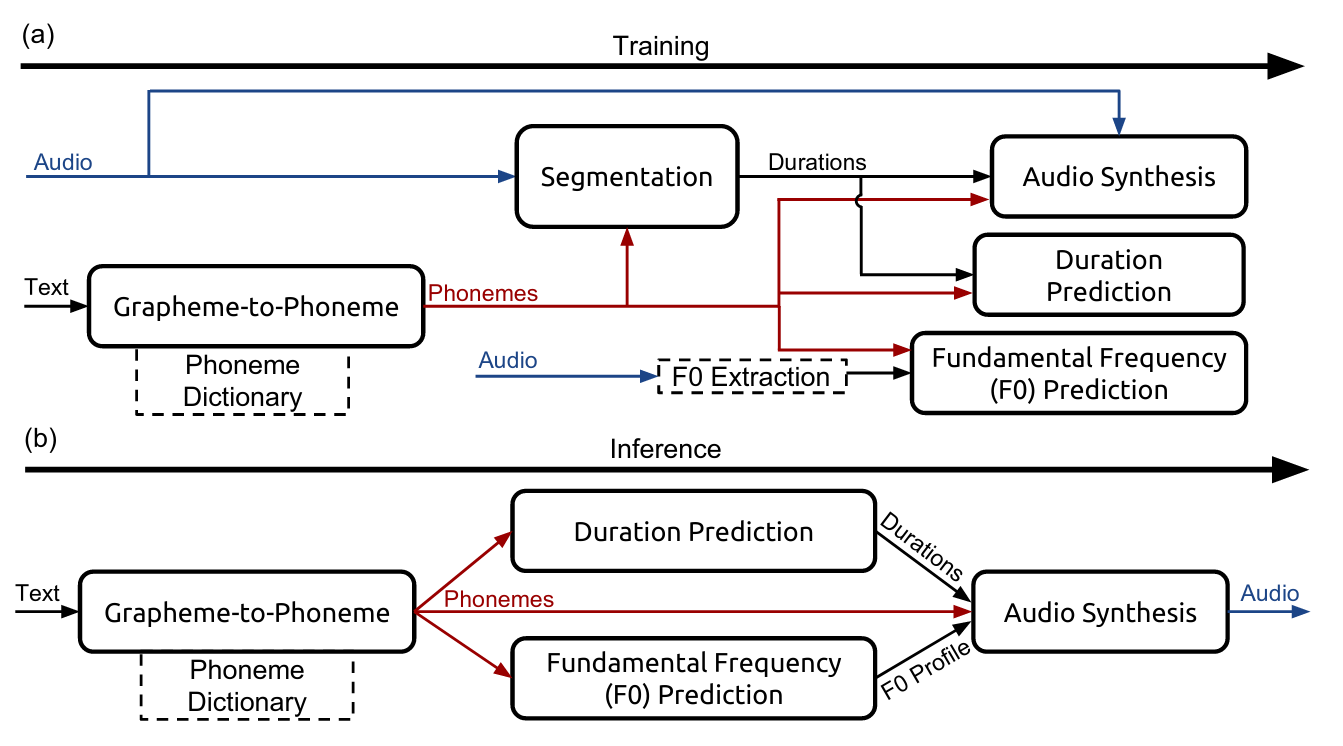
\includegraphics[width=14cm]{4_estado_del_arte_img/deepvoice_diagram.png}
\end{center}

En los modelos donde cada componente existe como una caja negra que solamente recibe una entrada y ofrece una salida, los errores se van acumulando en cascada sin que pueda existir una retroalimentación ni en la fase de entrenamiento ni en la fase de inferencia.

\subsection{Sistemas extremo a extremo bipartitos}

Estos sistemas reutilizan vocoders existentes también entrenados para ensamblarse como un sistema completo, pero su componente principal no podemos considerarlo un sistema de texto a voz completo sino un sistema de texto a espectrograma, siendo este espectrograma la entrada del vocoder.

Entre los vocoders habituales encontramos WaveNet, que ya se empleaba en el sistema mucho más modularizado de Deepvoice.

\subsubsection{Tacotron}

Poco después de la publicación del modelo Deep Voice, otro equipo de investigadores de Google publicaron el primer modelo \hyperref[EA_5]{[7]} que afirmaba ser un sistema TTS end-to-end: Tacotron.

Prácticamente a partir de este punto todos los autores afirman que su modelo funciona extremo a extremo, aunque dicha afirmación debe ser tomada con cautela. Es cierto que Tacotron tiene una arquitectura mucho más cohesionada que Deep Voice, donde la mayoría de componentes relevantes conforman un único modelo entrenado.

\begin{center}
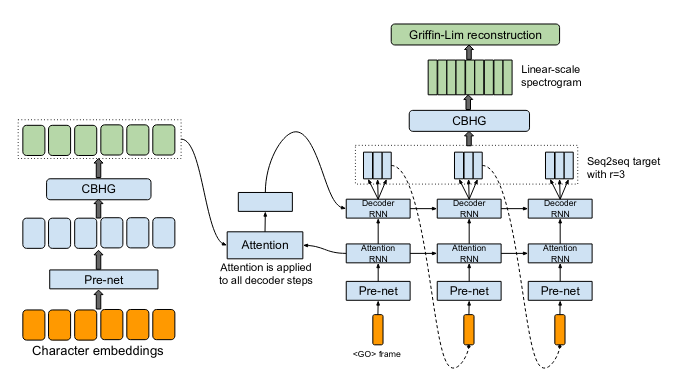
\includegraphics[width=14cm]{4_estado_del_arte_img/tacotron_0.png}
\end{center}

Pero la salida propiamente del modelo es un espectrograma y el componente final que transforma dicho espectrograma en una forma de onda no es entrenable. En la publicación original se dice:

\begin{displayquote}

«While Griffin-Lim is differentiable (it does not have trainable weights), we do not
impose any loss on it in this work. We emphasize that our choice of Griffin-Lim is for simplicity; while it already yields strong results, developing a fast and high-quality trainable spectrogram to waveform inverter is ongoing work.»

\end{displayquote}

Aún así, este modelo abrió la puerta a todos los desarrollos actuales basados en modelos cada vez más avanzados y aspirando cada vez más a incorporar más y más componentes para se efectivamente end-to-end.

Otra de las características significativas de este modelo es el uso de una arquitectura codificador-decodificador con un paradigma basado en atención. Esto supone que el modelo tiene una etapa intermedia donde la entrada de datos se codifica a una representación intermedia que luego se decodifica para generar el resultado deseado.

Esta etapa de compresión de datos además emplea un paradigma de atención, que en reglas generales supone el remarque de cierta información sobre otra en base a un criterio (temporal, espacial, etc...) para "atender" a lo más relevante a la hora de entrenar el modelo.

La representación adecuada de la información en estos estados internos para una efectiva comunicación entre en codificador y el decodificador es lo que entendemos por alineamiento en la etapa de entrenamiento y suele representarse con diagramas como este.

\begin{center}
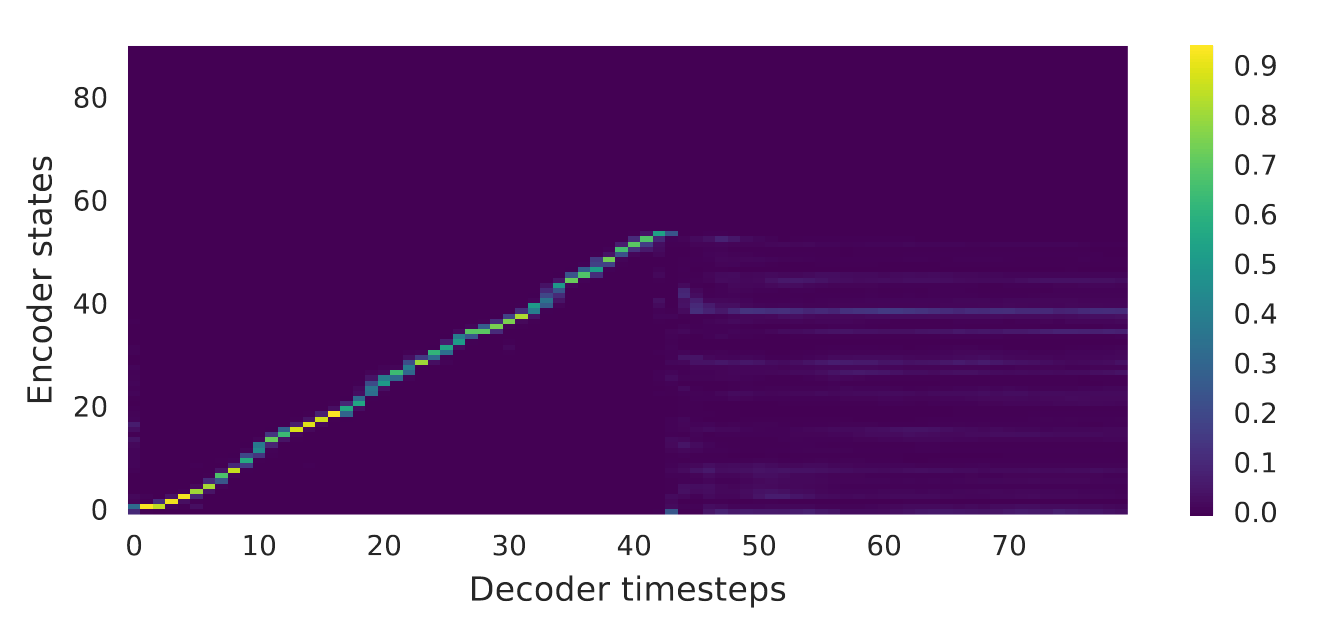
\includegraphics[width=14cm]{4_estado_del_arte_img/tacotron_1.png}
\end{center}

\subsubsection{Tacotron 2}

Del mismo equipo de ingenieros de Google llegó un año después de la publicación de Tacotron la siguiente iteración \hyperref[EA_6]{[8}, donde mejoran la arquitectura anterior y sobre todo abordan un mejor vocoder, uno de los puntos más flojos de Tacotron.

En este caso el vocoder pasa a ser un modelo entrenado llamado WaveNet  \hyperref[EA_7]{[9]}. Este modelo generativo de audio emplea un tipo de red RNN con convoluciones dilatadas que permiten reducir el número de capas ocultas y la cantidad de conexiones.

\begin{figure}[H]
\centering
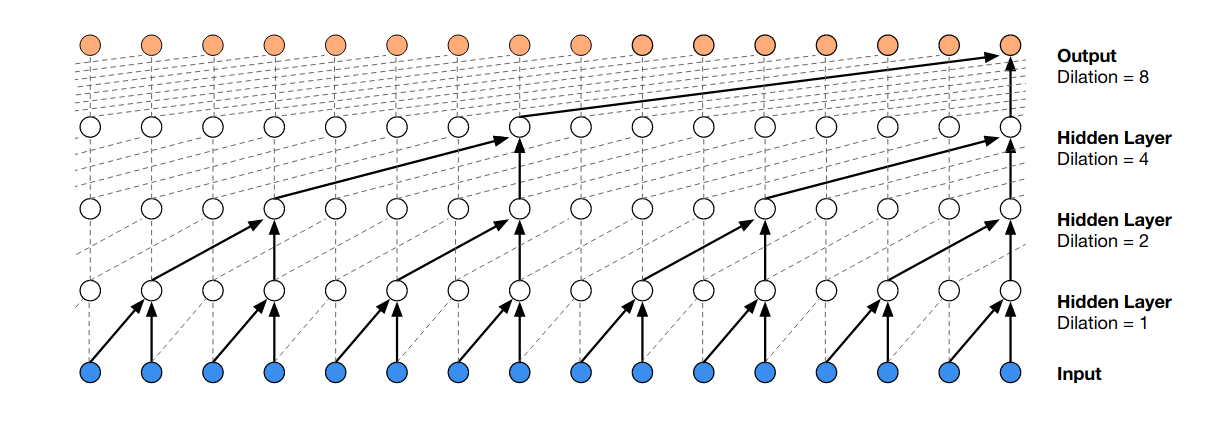
\includegraphics[width=14cm]{4_estado_del_arte_img/wavenet_0.png}
\caption{Diagrama del modelo WaveNet.}
\label{fig:figure1}
\end{figure}

Sus autores apuntan algo que más arriba habíamos mencionado ya, estos modelos precisan de poco o ningún conocimiento del dominio de la síntesis de voz para obtener resultados mejores que los modelos paramétricos que habían precisado una labor inmensa de ingeniería de características.

\begin{displayquote}
«The resulting system synthesizes speech with Tacotron-level prosody and WaveNet-level audio quality. This system can be trained directly from data without relying on complex feature engineering, and achieves state-of-the-art sound quality close to that of natural human speech.»
\end{displayquote}

Por lo demás Tacotron 2 conserva las características fundamentales de la arquitectura de Tacotron pero la incorporación de un vocoder mejor supone una mejora notable de la calidad de audio final. 


\begin{figure}[H]
\centering
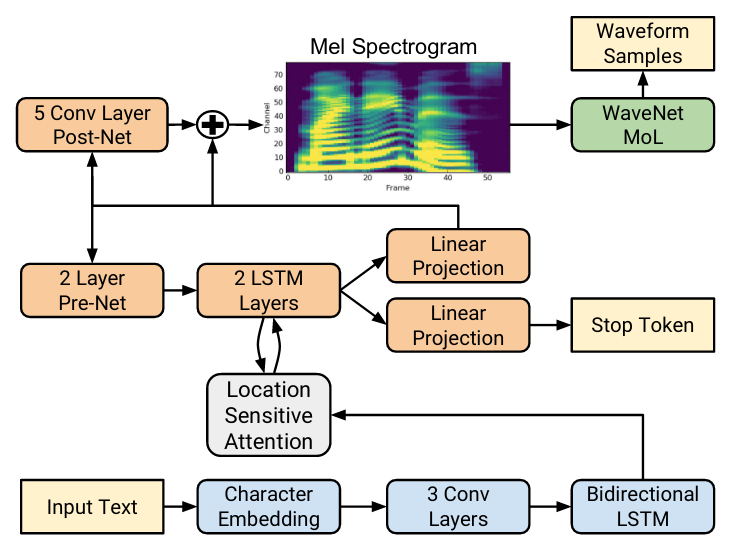
\includegraphics[width=12cm]{4_estado_del_arte_img/tacotron2_0.png}
\caption{Diagrama del modelo Tacotron 2.}
\label{fig:figure1}
\end{figure}


\subsection{Sistemas extremo a extremo monolíticos}

Se trata de sistemas completamente extremo a extremo, sin tener componentes desarrollados de forma independiente como el caso de Tacotron y Tacotron 2. Esto no significa que no puedan identificarse diferentes elementos o componentes en el modelo, lo que significa es que estos componentes están estrechamente relacionados y se pueden entrenar como uno solo.

\subsubsection{VITS}

Este es el modelo presentado a mediados de 2021 supone un gran salto frente a modelos anteriores basados en dos componentes conectados mediante una representación de características lingüísticas o bien un espectrograma tipo MEL.

VITS (Variational Inference with adversarial learning for end-to-end Text-to-Speech)  \hyperref[EA_8]{[10]} presenta un sistema realmente end-to-end que consigue dar solución a la dificultad de entrenar modelos donde se encadenan muchos elementos en cascada. 

Otros modelos antes que VITS intentaron hacer una propuesta de un sistema completo, extremo a extremo, pero la falta de paralelización en sus propuestas suponía un problema de rendimiento importante. Este podría ser el caso de Transformer TTS, que intentó adaptar un modelo de gran éxito en otros ámbitos NLP.

La arquitectura de VITS integra en un mismo modelo también el vocoder responsable de la generación final de sonido, además de otras características como un generador estocástico que permite a partir de una misma entrada generar resultados distintos.


\begin{figure}[H]
\centering
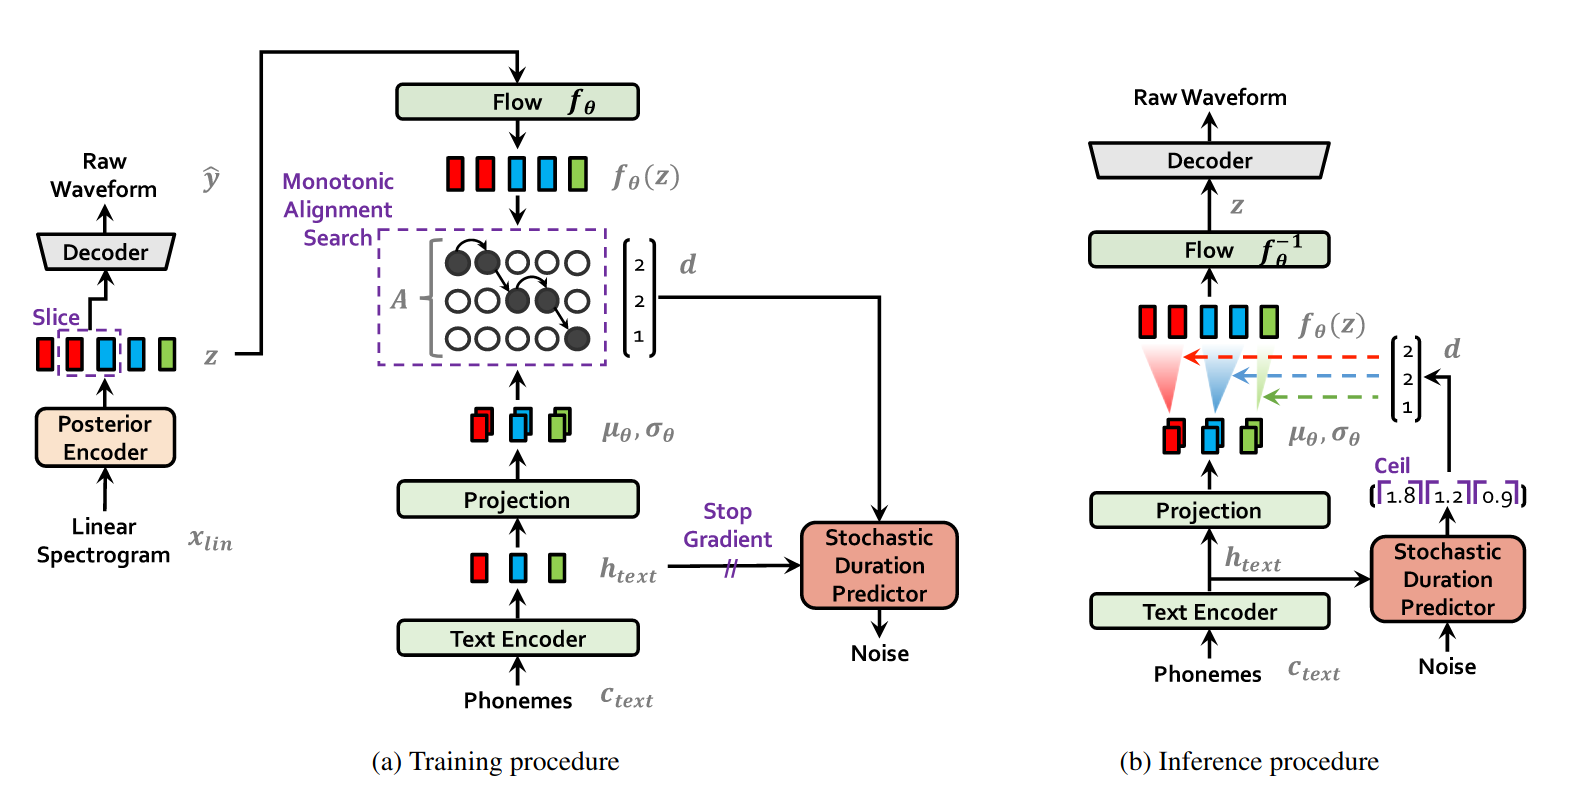
\includegraphics[width=14cm]{4_estado_del_arte_img/vits_0.png}
\caption{Diagrama del modelo VITS.}
\label{fig:figure1}
\end{figure}


VITS también permite entrenar simultáneamente un conjunto de hablantes distintos para obtener un único modelo final que permitirá seleccionar el hablante sobre el que realizar la inferencia. 

El motivo por el cual el entrenamiento de modelos en general requiere de unidades de procesamiento que explotan el paralelismo masivo como las GPUs o que además tienen hardware especialmente diseñado como las TPU o NPU, es porque no existe otra forma de acelerar la ingente cantidad de cálculos que requiere esta tarea.

Un modelo que no tenga posibilidades de ser paralelizado no es un modelo viable en la actualidad, por eso este modelo a efectos prácticos y probables representa el estado del arte en la síntesis de voz a partir de texto.

\subsection{Sistemas con características adicionales}

Hasta el momento hemos visto únicamente modelos que parten de cero, es decir, que son entrenados mayormente sobre un dataset particular y ofrecerán inferencias con lo aprendido al haber sido entrenados sobre dicho dataset.

Algunos desarrolladores han experimentado continuando el entrenamiento anterior sobre un dataset nuevo con la idea de conseguir una voz particular sobre un dataset mucho mayor con una voz distinta, pero los resultados de esto son dispares y no se han encontrado publicaciones serias al respecto. 

Esta forma de trabajar es lo que se denomina transferencia de aprendizaje, una técnica empleada en otros ámbitos del Aprendizaje Computacional.

\subsubsection{YourTTS}

Hace apenas unos meses se publicó este nuevo modelo  \hyperref[EA_9]{[11]} que se construye sobre la arquitectura base de VITS y aspira a permitir realizar una adaptación a un hablante nuevo en la etapa de inferencia y no en el propio entrenamiento.

Este modelo da un paso más allá y nos acerca en gran medida a tender puentes realistas hacia la generación de deepfakes sin grandes conocimientos técnicos ni gran esfuerzo\footnote{Esto es algo que preocupa a los autores de esta publicación, tanto es así que públicamente rechazan en estos momentos dar consejos ni detalles sobre ajustes finos del modelo para gente fuera de la comunidad investigadora. \url{https://github.com/Edresson/YourTTS/issues/5}}.

Por desgracia lo prometedor de este modelo no es algo que hayamos podido explotar en este trabajo, al depender sus resultados de un entrenamiento bastante amplio de VITS con múltiples hablantes, cosa que a día de hoy no existe en castellano.

Los autores de esta publicación afirman que con una muestra de menos de un minuto de voz se puede conseguir un clonado aceptable:

\begin{displayquote}
«Require less than 1 minute of speech to fine-tune the model for speakers who have voice/recording characteristics very different from those seen in model training, and still achieve good similarity and quality results»
\end{displayquote}

Aún sin haber podido probar lo cierto o falso de dicha afirmación, otras afirmaciones previas en este ámbito han probado tener una tendencia a la hipérbole y a centrar la atención en los casos ideales y no en los resultados habituales.

\subsection{Toolkits}

La proliferación de numerosos modelos y variaciones de los mismos presenta un reto a la hora de pasar de la investigación académica a la implementación de sistemas reales en producción. 

Muchos de los modelos arriba comentados además no siempre se acompañan con una implementación de referencia, o dicha implementación ha quedado tan obsoleta que otras implementaciones alternativas se vuelven la referencia de facto.

En esta situación se han constituido diversos toolkits que intentan encapsular muchos de estos modelos o componentes en un formato más accesible al integrador de sistemas o al usuario final. El ámbito de estos toolkits además no suele limitarse a los modelos de texto a voz en los que nos hemos centrado sino a otros ámbitos como el reconocimiento automático del habla.

\subsubsection{ESPnet}

El proyecto ESPnet  \hyperref[EA_2]{[12]} se define a sí mismo como:

\begin{displayquote}
«ESPnet is an end-to-end speech processing toolkit covering end-to-end speech recognition, text-to-speech, speech translation, speech enhancement, speaker diarization, spoken language understanding, and so on»
\end{displayquote}

Su objetivo es recopilar diferentes componentes para el procesamiento natural del lenguaje orientado a la síntesis de voz y la interpretación de la voz con el fin de crear un ecosistema que haga compatibles todos estos elementos e implementaciones.

Muchos de los modelos que hemos comentado anteriormente está integrados en ESPnet y hacer uso de ellos resulta así más sencillo y en cierto grado estandarizado.

\subsubsection{Coqui-AI}

De manera similar a ESPnet, Coqui-AI  \hyperref[EA_3]{[13]} es otro proyecto que aspira a generar un ecosistema que integre muchos de los desarrollos más actuales en el reconocimiento automático del habla así como en la síntesis de voz.

A diferencia de ESPnet, Coqui-AI tiene proyectos separados para los modelos TTS y los modelos ASR, por lo que el ecosistema es algo más pequeño y permite una curva de aprendizaje menos abrupta. En sus propios términos el proyecto afirma:

\begin{displayquote}
«TTS is a library for advanced Text-to-Speech generation. It's built on the latest research, was designed to achieve the best trade-off among ease-of-training, speed and quality»
\end{displayquote}

Este toolkit fue el que se decidió emplear para facilitar los entrenamientos de los modelos que finalmente se decidiesen entrenar. Hay dos grandes ventajas del uso de un entorno de este tipo: por una parte la base de código de los modelos ha sido mejor revisado y mantenido; por otra parte poder reutilizar herramientas para el entrenamiento como las necesarias para preparar el dataset reduce la cantidad de trabajo técnico específico para cada dataset.

\subsection{Conclusiones}

El estudio del Estado del Arte nos pone en situación de comprender el máximo punto de desarrollo de la investigación en el dominio que hemos definido para este trabajo, ahora conocemos no solo los modelos más avanzados para la generación de voz de forma sintética sino también algunos ecosistemas de herramientas que nos facilitarán dar pasos en la dirección de estudio que apuntaba la introducción de este proyecto de investigación. 

\newpage 
\newpage \section{Resultados}

\subsection{Resultados de investigación}

En esta sección se exponen los conceptos, lecciones y conclusiones más relevantes del proceso de investigación seguido como base para la posterior experimentación.

A diferencia del capítulo anterior donde razonábamos el Estado del Arte desde la perspectiva de lo interesante para las preguntas de investigación, aquí se exponen otros elementos que se han considerado necesarios comprender.

\subsubsection{Conceptos generales}

\paragraph{Atención} ~\\

Una de las primeras cosas que llamaron nuestra atención en la medida que se profundizaba en aspectos más técnicos de algunos de los modelos generadores de voz fue el concepto de atención. En términos generales entendemos atender como el acto de tomar en consideración a alguien o a algo particular respecto al resto al resto del entorno. 

Este concepto se aplica también al ámbito del Aprendizaje Computacional. En primer lugar es necesario aclarar que en general el entrenamiento de un modelo a partir de un conjunto de datos ya supone en cierto grado diferenciar la información relevante de aquella que no es significativa. Cuando hablamos de forma explícita de paradigmas o mecanismos de atención en un modelo determinado hablamos de forzar por diseño el peso de cierta parte de la información frente a otra.

Algunos modelos implementan mecanismos de atención especialmente relevantes, como los Transformer que se han hecho especialmente populares en años recientes en muchos problemas del procesamiento natural del lenguaje\footnote{Aunque no parece ser el caso en la síntesis de voz, pues la propuesta de Transformer TTS no obtuvo muy buenos resultados comparado con otras propuestas}.

Dependiendo de la forma de actuar de los diferentes mecanismos de atención podemos distinguir entre atención y auto-atención, siendo esta última bastante relevante en el modelo que hemos comentado:

\begin{displayquote}
«Self-attention, sometimes called intra-attention is an attention mechanism relating different positions of a single sequence in order to compute a representation of the sequence. Self-attention has been used successfully in a variety of tasks including reading comprehension, abstractive summarization, textual entailment and learning task-independent sentence representations»\hyperref[RES_1]{[14]}
\end{displayquote}

Debemos comprender que en los modelos tratados tenemos una entrada de datos como secuencia de longitud variable y una salida igualmente de longitud variable, esto se aborda con una arquitectura codificador-decodificador donde un mecanismo de atención es esencial.

Tacotron 2 emplea un mecanismo de atención especial basado en localización en la secuencia y en información temporal de pasos previos:

\begin{displayquote}
«We use the location-sensitive attention [...] which extends the additive attention mechanism to use cumulative attention weights from previous decoder time steps as an additional feature.»
\end{displayquote} \hyperref[EA_6]{[8]}

Por su parte VITS emplea el mismo mecanismo de atención de otro modelo anterior publicado por el mismo grupo de investigadores, llamado Glow-TTS \hyperref[RES_1]{[15]}:

\begin{displayquote}
«We follow the encoder structure of Transformer TTS with two slight modifications. We remove the positional encoding and add relative position representations into the self-attention modules instead»
\end{displayquote}

\paragraph{Alineamiento} ~\\

En los modelos basados en la arquitectura codificador-decodificador se precisa transformar una entrada de datos de longitud variable en una representación intermedia de tamaño fijo (codificar) para posteriormente transformar esta representación en una salida de tamaño variable (decodificar).

Durante el entrenamiento del modelo uno de los principales objetivos es encontrar la adecuada representación intermedia de los datos, encontrando en esa representación la relación entre la entrada y salida de datos. Este proceso es el que denominamos alineamiento en el modelo.

La evaluación de este alineamiento es una de las cosas que se ha tenido que prestar atención en el entrenamiento de los modelos, especialmente en el caso de Tacotron 2 que es menos robusto en ese sentido.

\begin{figure}[H]
\centering
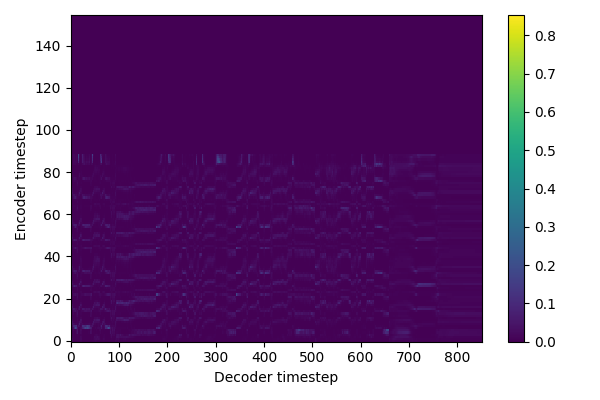
\includegraphics[width=10cm]{5_resultados_img/align-taco1.png}
\caption{Falta de alineamiento en un entrenamiento de Tacotron 2}
\label{fig:figure1}
\end{figure}

En esta figura podemos ver una fase muy temprana de entrenamiento de Tacotron 2 donde la representación intermedia de los datos es difusa.

\begin{figure}[H]
\centering
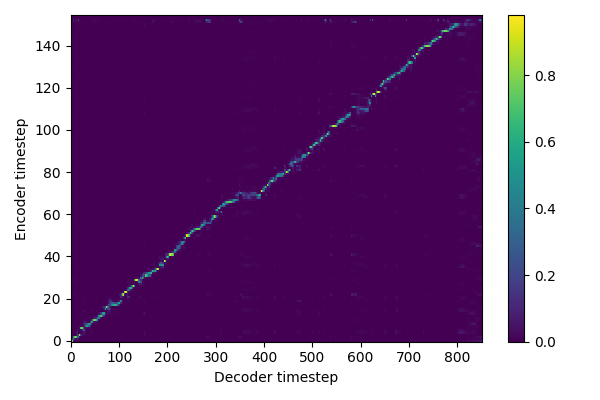
\includegraphics[width=10cm]{5_resultados_img/align-taco2.png}
\caption{Alineamiento definido en un entrenamiento de Tacotron 2}
\label{fig:figure1}
\end{figure}

El entrenamiento posteriormente progresó a un alineamiento notable, este es el resultado esperable pare el modelo Tacotron 2 con su arquitectura encoder-decoder particular.

\begin{figure}[H]
\centering
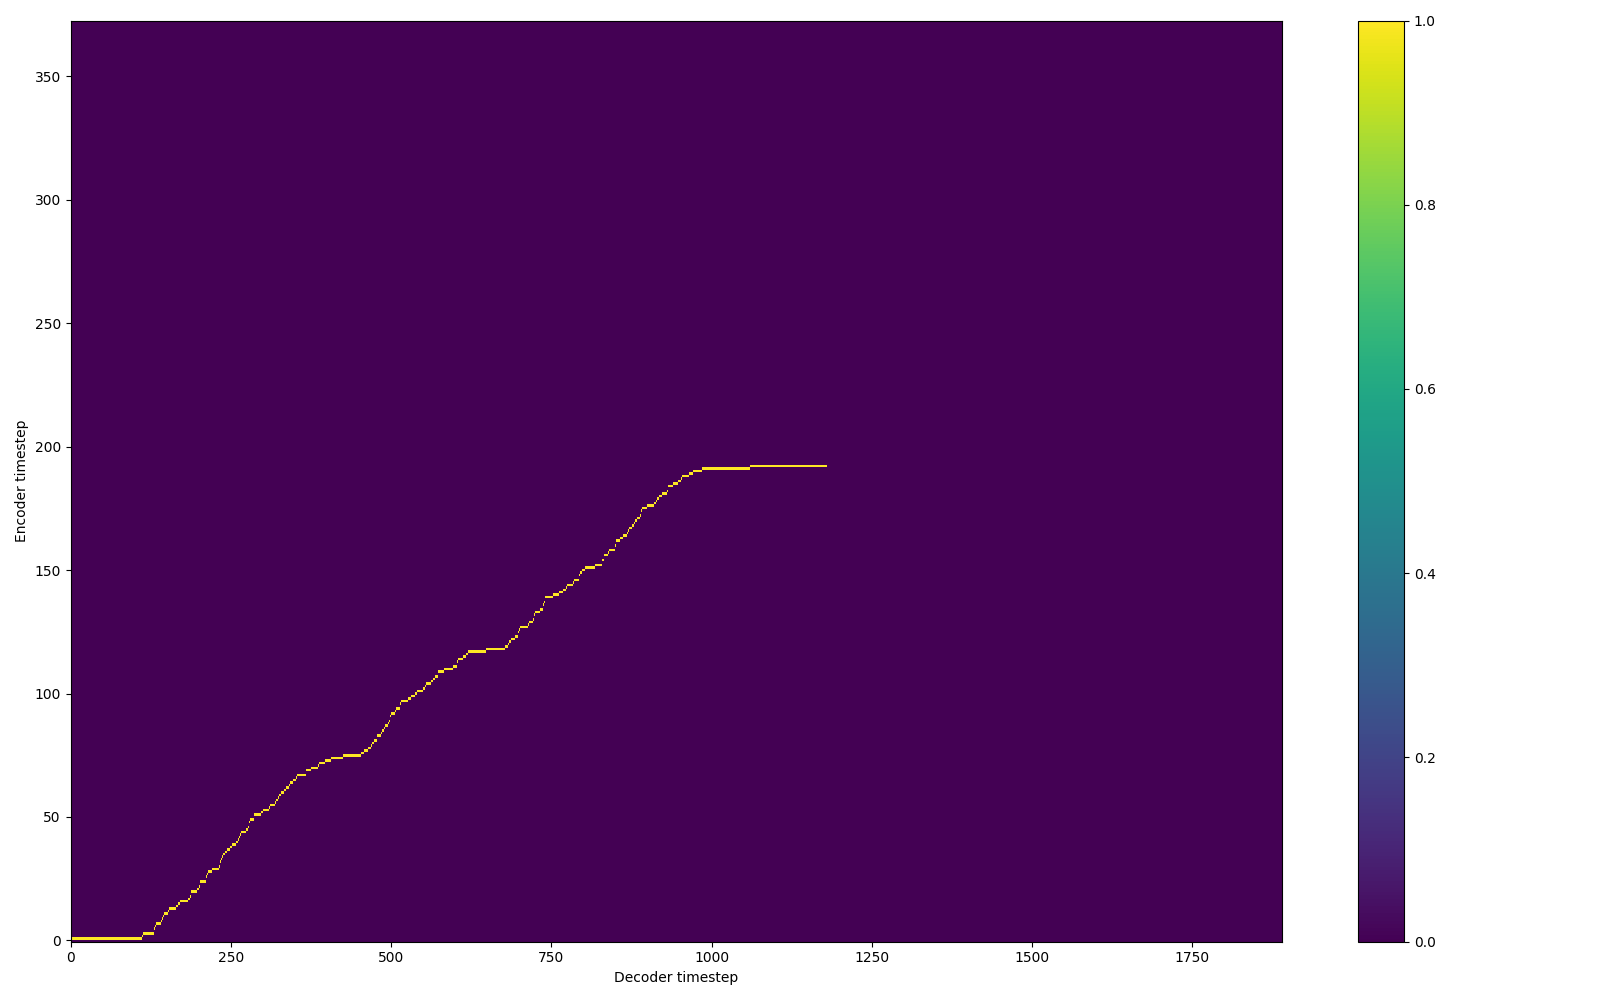
\includegraphics[width=10cm]{5_resultados_img/align-vits.png}
\caption{Alineamiento muy definido en el modelo VITS}
\label{fig:figure1}
\end{figure}

En este caso podemos ver como VITS es mucho más robusto en este aspecto, teniendo un alineamiento claramente definido.

\paragraph{Escala MOS} ~\\

Para todo problema que se aborda existe la necesidad de definir una escala que permita evaluar el grado de cumplimiento. En la mayoría de modelos estudiados esta métrica es la escala MOS (Mean Opinion Score), una métrica heredada de los sistemas de telefonía.

La escala MOS intenta medir la calidad de una comunicación de voz mediante la opinion media de los usuarios, su origen está en una recomendación de la International Telecomunication Union (ITU) publicada como P.800.1 \hyperref[RES_3]{[17]}.

En ella se define la escala como: 

\begin{displayquote}
«The value on a predefined scale that a subject assigns to his opinion of the performance of the telephone transmission system used either for conversation or for listening to spoken material»
\end{displayquote}

En la publicación también se comenta la posibilidad de definir la escala de forma objetiva, pero en los modelos revisados o no se dan más detalles del uso de esta escala o se comenta que se ha realizado una encuesta con muestras generadas.

Aunque esta escala nos ayuda a comprender las posibilidades de un modelo para generar voz de calidad no nos permite medir la calidad con la que el modelo imita la voz original del hablante y en qué grado permitiría generar una falsificación.

\subsubsection{Componentes y arquitecturas}

\paragraph{Modelos basados en RNN}

En el campo del Aprendizaje Computacional existen cada día más modelos y componentes de modelos distintos. El campo avanza a pasos agigantados cubriendo cada vez más categorías de problemas y encontrando mejores soluciones a problemas ya cubiertos con anterioridad.

En muchos problemas abordados el tamaño de la entrada de datos es fija o cuanto menos es fácilmente transformable a una entrada da datos normalizada sin perder información. Por ejemplo, en muchos problemas de Visión por Computador se traducen las imágenes a unas dimensiones determinadas en las cuales ha sido entrenado el modelo. 

En el caso de problemas de procesamiento natural del lenguaje, la entrada de datos es siempre de longitud variable y no existe una forma sencilla de preprocesar los datos para dimensionarlos a un tamaño fijo.


\begin{figure}[H]
\centering
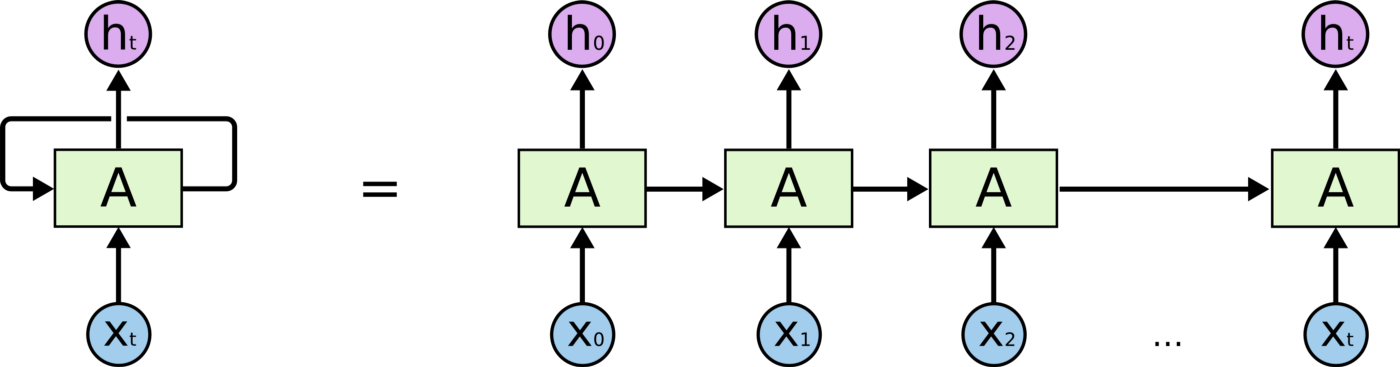
\includegraphics[width=10cm]{5_resultados_img/rnn-1.png}
\caption{Modelo RNN y su despliegue en un modelo secuencia.}
\label{fig:figure1}
\end{figure}

El uso modelos basados en redes neuronales recurrentes se vuelve entonces poco práctico \hyperref[RES_2]{[16]}, pues la complejidad de la red crece con el tamaño de la entrada de datos. Se hace necesario encontrar otras arquitecturas que puedan manejar la arbitrariedad del tamaño de los datos.

\paragraph{Modelos Codificador-Decodificador}

Se han mencionado ya varias veces con anterioridad para comentar características particulares o valoraciones del entrenamiento de algunos modelos, pero no hemos comentado en detalle lo que suponen los modelos codificador-decodificador (en inglés encoder-decoder o E/D). 

Partimos de una entrada de datos de longitud arbitraria, habitualmente una oración completa que traducir, analizar sentimientos, sintetizar voz o cualquier otra tarea similar. Si empleamos alguna arquitectura sencilla con perceptones y redes conectadas de forma simple, tendríamos que redimensionar la entrada de datos a un tamaño fijo con el cual el modelo ha sido entrenado. En otros modelos entenderíamos ese paso como una fase de normalización de los datos.

Pero no existe ninguna forma sencilla de normalizar información en formato textual a una dimensionalidad determinada y una expresión única. Tenemos además el problema añadido de que el lenguaje natural tiene múltiples formas de expresar información equivalente. Es cierto que existen formas matemáticas\footnote{Habitualmente en modelos que tienen vectores de N dimensiones donde cada palabra tiene un valor para cada dimensión del vector. Por ejemplo GloVe o word2vec son modelos así.} de representar palabras, por ejemplo haciendo uso de word embeddings, pero si combinamos los valores en un vector final la información se va diluyendo.

\begin{figure}[H]
\centering
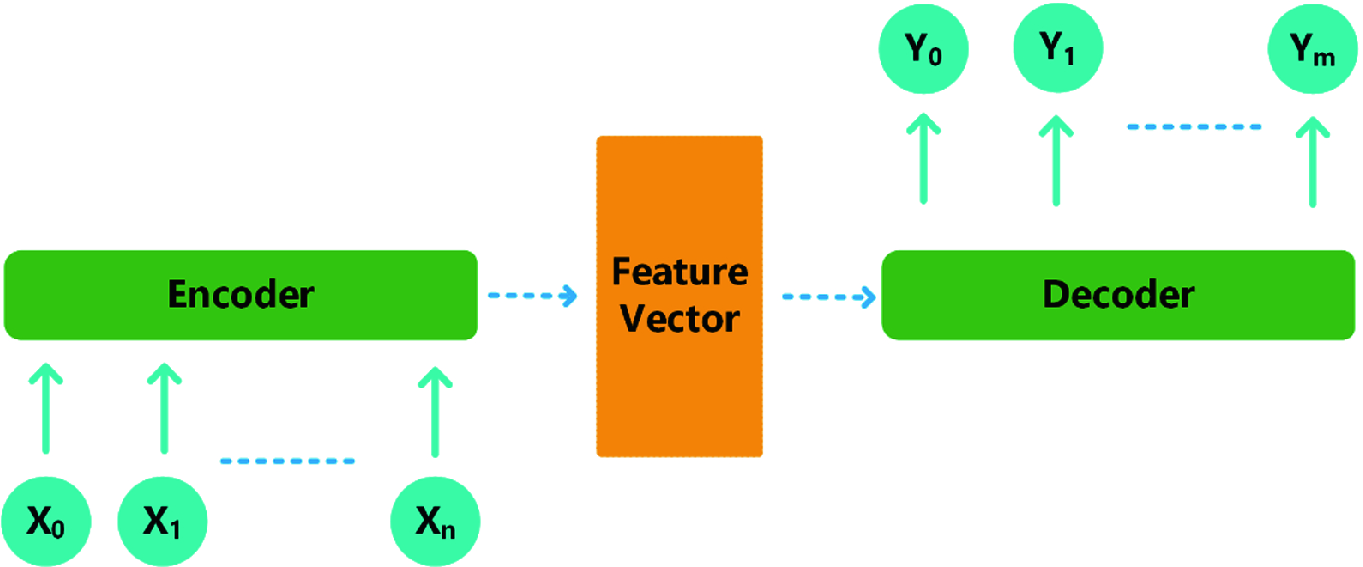
\includegraphics[width=14cm]{5_resultados_img/e-d.png}
\caption{Representación abtracta de un modelo codificador-decodificador.}
\label{fig:figure1}
\end{figure}

Necesitamos alguna forma de identificar la información más relevante en una oración determinada y al mismo tiempo mapear esa información a un estado oculto intermedio en el modelo. Ese es el paradigma de estos modelos codificador-decodificador, pero la forma en la cual se mapea esa información en un estado intermedio es un nuevo problema que puede tener muchas soluciones.

Dentro de las soluciones a este problema precisamente aparecen los dos conceptos que hemos definido anteriormente: atención y alineamiento. Un mecanismo de atención lo que nos permite es representar la información relevante en una entrada de forma y longitud variable. Para ello podemos confiar en las relaciones entre las diferentes palabras (auto-atención) o en otras cuestiones de localización o temporalidad de la entrada de la secuencia de datos (atención).

Muchos de los cambios y avances de los modelos revisados parten de revisar y abordar este problema desde una perspectiva distinta o con ajustes añadidos. 

Como habíamos comentado más arriba, durante el proceso de entrenamiento de estos modelos, una de las métricas que debemos observar para evaluar el avance del entrenamiento es el alineamiento. Esto implica que efectivamente conseguimos representar la información de entrada fielmente en el estado intermedio y que el decodificador consigue reconstruir a partir de esta representación la salida esperada del modelo.

\subsubsection{Datasets}

Para realizar el entrenamiento de los modelos contemplados es necesario conseguir datos del perfil de voz de la persona en un formato particular. Ninguno de los modelos abordados contempla el uso de conjuntos de datos de más de un hablante, por lo que nos ceñiremos a los datasets de una sola persona.

Los datos en este dataset deben presentarse como una serie de parejas de sonido y su transcripción textual en el idioma que se aborde. El formato particular para realizar el emparejamiento varía, aunque es habitual que se presente como un conjunto de clips de sonido y un fichero de datos CSV o TSV que los empareja con su transcipción.

Las características de estos datasets pueden determinar en gran medida el éxito del entrenamiento del modelo. El proyecto Mozilla TTS \hyperref[RES_4]{[18]} lista los siguientes puntos de atención para obtener un dataset de buena calidad:

\begin{itemize}
    \item Variedad en longitud de los fragmentos de audio: se sugiere una distribución gaussiana de la longitud de los clips.
    \item Ausencia de errores de transcripción: coincidencia entre los fonemas vocalizados y su representación textual en esa lengua.
    \item Grabaciones de calidad sin ruido: claridad, falta de distorsión, sonidos de fondo o ruido base.
    \item Tono y velocidad homogéneos entre clips: pronunciación neutra y constante en todos los fragmentos.
    \item Adecuada cobertura de fonemas: deben incluirse muestras que cubran todos los fonemas posibles del idioma.
    \item Naturalidad: pausas y entonación adecuada.
\end{itemize}

Algunas de estas características se han tenido especialmente en cuenta, otras de las recomendaciones son demasiado subjetivas para poder cuantificarse y especialmente para cuantificarse entre diferentes idiomas.

Se han generado algunas métricas concretas de varios datasets que se encuentran en el anexo \hyperref[Análisis de datasets]{Análisis de datasets}.

\subsubsection{Herramientas comerciales}

Algunas herramientas comerciales que hacen uso de algunas características de estos modelos han ido apareciendo con el tiempo, pero no suelen cumplir la función de síntesis de voz entrenable que realmente cuadra con los objetivos del proyecto.

De las diversas herramientas y webs probadas, prácticamente ninguna realmente ofrece algo adaptable, únicamente Resemble.ai ofrece algo similar. Esta web promete un modelo de voz luego de haber grabado 50 fragmentos de audios mediante su interfaz. El problema es que únicamente acepta inglés como idioma en su versión gratuita.

Otra web que ofrece algunas características prometedoras es fakeyou.com, quizá lo más cercano a lo que hemos investigado y experimentado, pero no se ha llegado a profundizar en el uso de esta web ya que se encontraron problemas con ella durante las pruebas de uso. 

Esta web sí que positivamente lista en la descripción de su misión y funcionamiento alguno de los modelos que hemos estudiado, como Tacotron 2.

\subsection{Resultados de experimentación}

En este apartado entramos a detallar los resultados de los diferentes experimentos realizados, tanto en lo positivo como en los errores, fallos y limitaciones encontrados en el proceso.

\subsubsection{Datasets}

Aunque existen ya datasets de voz en castellano con los que algunos de los modelos vistos se han podido entrenar, para conseguir el objetivo de entrenar un modelo con la voz propia se ha decidido generar un dataset propio.

Se ha intentado mantener cierta homogeneidad en el tiempo de los fragmentos, pues el tamaño de los mismos condiciona las necesidades de memoria en el entrenamiento de los modelos y unos tiempos cercanos aseguran que el entrenamiento podrá aprovechar al máximo los recursos de hardware sin eventualmente encontrar errores por falta de memoria.

Algunos detalles más técnicos sobre la grabación de audio se puede localizar en el \hyperref[Grabación de datasets]{Anexo 11.1}. El resultado final en forma de dataset se encuentra documentado en la sección \hyperref[Entregables]{8. Entregables}.

\paragraph{Primera iteración} ~\\

En una primera iteración de la generación de este dataset y posteriormente su uso como datos de entrenamiento se identificaron varios problemas. El más importante de ellos fue la ausencia de ciertos fonemas en el conjunto de entrenamiento. 

No se usó ningún criterio particular para la selección de los fragmentos de texto a grabar y como era esperable en cierto grado se reprodujo la tabla de frecuencias de los fonemas del castellano. El problema de esto es que ciertos sonidos le costarían mucho al modelo aprenderlos o no los aprendería en absoluto.

Adicionalmente en esta primera prueba apenas se grabaron 30 minutos de audio en 130 fragmentos, lo que hacía que la muestra de fonemas fuese aún más pobre en algunos casos.

\paragraph{Segunda iteración} ~\\

En esta segunda iteración se emplearon técnicas similares a las anteriormente mencionadas pero se tuvo especial atención al ruido ambiental. Se hizo manifiesto que este ruido se trasladaba a los resultados del modelo y en algunos casos se amplificaba haciéndose mucho más notable. 

Además de buscar un entorno menos ruidoso se incorporaron mecanismos de redacción de ruido adicionales con lo que la calidad mejoró.

Se grabaron un total de 500 frases y se amplió la longitud máxima de las mismas a 50 palabras (anteriormente se había fijado en 24) esperando así mejorar la inferencia de textos más largos.

Adicionalmente se optó por mantener las grabaciones de sonido con la calidad original de muestreo de 48kHz en lugar de 22kHz que es la habitual en estos datasets destinados al entrenamiento de modelos de síntesis de voz.

\subsubsection{Modelos}

En la revisión del estado del arte se identificaron muchos modelos distintos susceptibles de ser probados y entrenados con el dataset de voz propio que se estaba generando, pero el entrenamiento de modelos resulta costoso en tiempo y recursos.

En general el tiempo de entrenamiento de cada modelo ha variado entre 3 días y una semana en local y siempre más de una semana en Google Colab. Sobre las dificultades para entrenar modelos en Google Colab y las posibles soluciones se ha redactado un \hyperref[Entrenamiento en Google Colab]{anexo específico}.

Esto ha supuesto la obligación de elegir un solo modelo en el que centrar el grueso del tiempo y recursos disponibles para este trabajo. El modelo finalmente elegido fue VITS por posicionarse como el que mejores resultados ofrece con los datos actuales y que al mismo tiempo tenga una implementación abierta.

Antes de que se tomase esta decisión se comenzaron a hacer pruebas de entrenamiento con Tacotron 2 poco satisfactorias, aunque también se considera relevante documentarlo.

\paragraph{Tacotron 2} ~\\

En una etapa temprana de desarrollo del proyecto se comenzó a revisar el código del modelo Tacotron 2 en la implementación que NVIDIA había hecho pública \hyperref[RES_5]{[19]}. Se encontraron bastantes problemas por incompatibilidades de software.

Todo el código que se ha trabajado en este trabajo se ha realizado en Python y empleando algunas librerías para Aprendizaje Computacional como son TensorFlow o (Py)Torch. Para que el software de un modelo funcione adecuadamente tiene que existir compatibilidad entre estos elementos:

\begin{enumerate}
    \item Intérprete de Python
    \item Implementación del modelo en código
    \item Librerías que use la implementación
    \item Lenguaje/arquitectura de aceleración
    \item Drivers de la GPU
    \item GPU
\end{enumerate}

En proyectos cuyo código se encuentra adecuadamente mantenido no suele haber problemas, pero este proyecto había publicado su implementación hace unos 4 años y no se ha mantenido demasiado actualizado el código en línea con las dependencias que tenía.

Particularmente encontramos que la versión de Torch que se instala por defecto al instalar los requisitos del repositorio no es compatible con la GPU del sistema. Fue necesario instalar una versión especial que sí implementa compatibilidad con las últimas tarjetas gráficas de NVIDIA. Más detalles sobre esto se encuentran en el anexo \hyperref[Entorno de entrenamiento]{Entorno de entrenamiento}.

Una vez subsanados los problemas más técnicos se inició un entrenamiento con el dataset LJSpeech, que progresivamente devolvió resultados aceptables de síntesis de voz


\paragraph{VITS} ~\\

En términos de experimentación gran parte del esfuerzo se volcó en este modelo, habiéndose realizado con él numerosos experimentos. En un primer momento se hizo revisión de la base de código originalmente publicada \hyperref[RES_6]{[20]} por los autores del modelo, pero finalmente se trabajó con la implementación del toolkit Coqui-AI.

Una de la primeras cosas que nos dimos cuenta trabajando con este modelo fue la robustez con la que se progresaba hacia un alineamiento muy definido, algo que había sido relativamente problemático con Tacotron 2 como se había comentado más arriba cuando hablábamos de este concepto.

\begin{figure}[H]
\centering
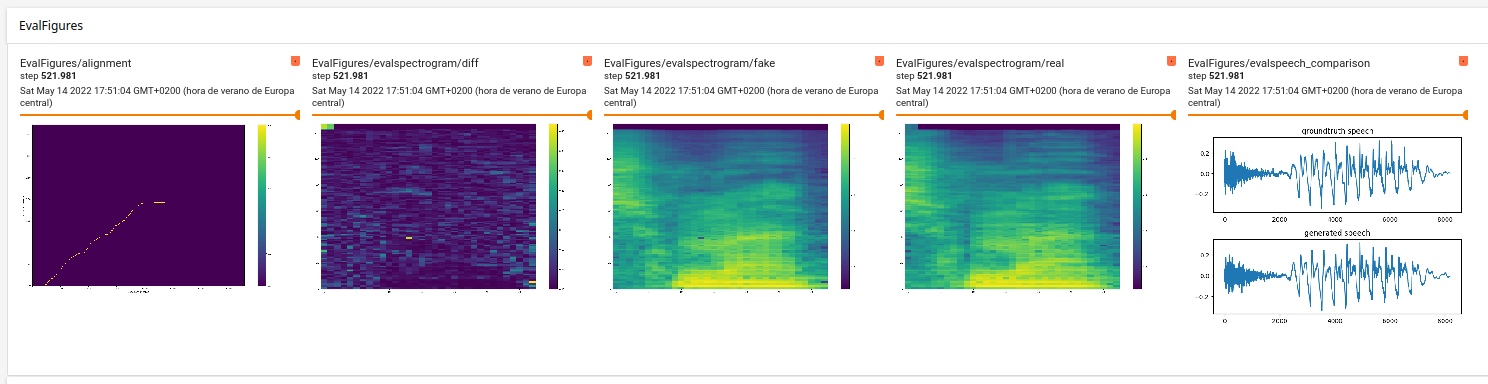
\includegraphics[width=14cm]{5_resultados_img/vits-2.png}
\caption{Alineamiento junto a otras métricas en TensorBoard.}
\label{fig:figure1}
\end{figure}

Durante los entrenamientos el seguimiento del progreso se ha realizado empleando una herramienta llamada TensorBoard, que permite visualizar la progresión de algunos estados internos del modelo, métricas y muestras de generación. Los registros de estos entrenamientos se presentan también como entregables.

Una vez que pudimos reproducir los resultados de entrenamiento en inglés comenzamos a hacer los ajustes necesarios en el modelo para poder trabajar con castellano. Entre los cambios se incluyen:

\begin{itemize}
    \item Ampliar la lista de caracteres reconocidos por el modelo
    \item Ajustar la lista de fonemas posibles
    \item Ajustar el reemplazo de ciertos caracteres especiales por su nombre
\end{itemize}

Parte de este trabajo se puede encontrar en un \href{https://github.com/daniel-dona/coqui-ai-TTS}{fork} específico del repositorio de Coqui-AI.

Con ello se pudo realizar un primer entrenamiento cuando el dataset aún contenía poco más de 100 registros grabados. En este punto existían aún bastantes errores de síntesis en ciertas palabras, aunque en cambio otras se sintetizaban sin problema. En este punto empezamos a sospechar la posibilidad de que se estuviesen generando fonemas en las inferencias que no estaban en el dataset\footnote{Algunos elementos más sobre esto se encuentran en el anexo sobre Análisis de Datasets}.

Una vez se generó el dataset más amplio de 500 registros se consiguieron resultados bastante mejores, sin apenas errores de pronunciación en las inferencias generadas. A partir de ese momento se comenzó a valorar el realizar ajustes de hiperparámetros del modelo en la búsqueda de obtener aún mejores resultados.

Se valoraron los siguientes parámetros:

\begin{itemize}
    \item Tamaño de lote y tasa de aprendizaje
    \item Canales MEL y frecuencia de muestreo
    \item Fonetizador
\end{itemize}

El primer parámetro fue de ajuste obligado pues la GPU empleada en la mayoría de entrenamientos (local) solo disponía de 12GB de memoria y no toda disponible. El tamaño de lote es un valor que ajusta cuántas muestras del dataset se cargan y procesan de forma simultánea.

Un problema encontrado al realizar este ajuste es que el tamaño ocupado en memoria no es siempre el mismo, al variar la longitud de los registros de audio, por lo que debemos establecer valores prudentes. A la par que reducimos el tamaño de lote debemos ajustar de forma acorde la tasa de aprendizaje, pues estamos modificando los pasos de entrenamiento del modelo.

También hay que tener en cuenta que este modelo ajusta dinámicamente la tasa de aprendizaje según progresa el entrenamiento, nosotros solo establecemos un valor inicial. En general este valor no es crítico, un valor muy alto puede hacer que el modelo apenas progrese y un valor muy bajo puede hacer que el entrenamiento caiga en un mínimo local del que no pueda salir, pero existe un rango de valores que posiblemente funcionen y permitan un buen entrenamiento.

El siguiente parámetro define una representación interna del modelo, posterior al decodificador, que emplea espectrogramas MEL como forma de representación del sonido generado. Esta es la representación que consumirá el vocoder (sea externo o integrado en el modelo) y a partir de donde se generará la forma de onda final.

Un espectrograma MEL se caracteriza por emplear diferentes filtros por bandas de frecuencias para reconstruir finalmente una onda sonora. Por defecto el modelo emplea 80 bandas, ya que también planeábamos subir la frecuencia de muestreo a 48kHz desde los 22.5kHz originales era apropiado también subir a 128 bandas MEL.

Aunque es habitual emplear frecuencias de muestreo bajas para la reproducción de voz humana por lo más limitado de las frecuencias empleadas, una mayor tasa de muestreo permite reproducir un rango de frecuencias mayor y con ello intuíamos reducir ciertas pérdidas de calidad. El resultado de estos cambios fue modesto, aunque sí se logró mantener algo más de calidad en los graves de las muestras de audio generadas.

Por último, decidimos experimentar con el componente que convierte los grafemas en fonemas dentro del modelo. Aquí sí encontramos diferencias notables. Mientras que si el modelo únicamente toma caracteres alfabéticos como entrada apenas tenemos una treintena de casos, cuando se pasan al fonemizador obtenemos bastantes más variantes.

Esto es así porque fonemizadores como eSpeak son capaces de incluir no solo los fonemas de forma plana sino también indicar variantes de estrés en ciertos fonemas y en cierto grado incluso información sobre la entonación. Esto, con un dataset que cubra sobradamente todos los casos es algo positivo, pero en uno más escueto como el nuestro supone una cobertura solo parcial de los casos.

Cuando pidamos al modelo entrenado con estos fonemas una palabra que contenga una variante desconocida o poco presente en el dataset encontraremos un error de síntesis o una calidad degradada en ese punto. Para el modelo que entrenamos estas variaciones constituyen símbolos distintos y aunque supongan una pequeña variación de otro fonema mucho más común el aprendizaje de uno no se aplica al otro.

Decidimos entonces realizar una prueba suprimiendo este paso, entrenar el modelo dando por entrada los caracteres textuales en lugar de una representación fonética. En nuestro caso de esta forma de obtenían resultados algo mejores, sin errores de pronunciación identificables. Tanto fue así que decidimos incluir esta variante en los entregables y en las muestras generadas para poder compararse.

La explicación de esta mejora es que los mecanismos de atención del modelo son suficientes para identificar las variantes de pronunciación de un grafema particular en una palabra, con ello se vuelve innecesario el paso previo de convertir el texto a una representación fonética. Pero en estas implementaciones el fonetizador se emplea para una tarea adicional, convertir otros símbolos no alfabéticos a una representación textual: nombres de símbolos, cifras cardinales u ordinales y otros.




\newpage 
\newpage \section{Discusión}

A la luz de los resultados expuestos podemos ahora evaluar y discutir en qué medida se han cubierto las expectativas proyectadas al inicio de este trabajo de investigación.

Los problemas aquí expuestos no son necesariamente calco exacto de aquellos inicialmente delineados, pues en el propio desarrollo del trabajo existe margen de reformulación de algunos de ellos siempre respetando los límites de las tesis de partida.

Esto supone además el planteamiento de nuevos problemas, resueltos o no resueltos, a raíz del avance del trabajo, así como la síntesis de todo esto en líneas de investigación tanto del trabajo como futuras\footnote{Las líneas futuras se exponen en el capítulo de Conclusiones}.

\subsection{Problemas resueltos}

\subsubsection{Identificación del Estado del Arte}

En un trabajo de investigación de estas características, donde se aborda un tema o problema de incipiente actualidad, es crucial tener el mejor y más actualizado conocimiento del dominio sobre el que se trabaja. Identificar los últimos avances era una tarea sin la cual el resto del trabajo no sería posible, o sería posible pero dejando en el tintero muchos aspectos.

La dinámica de avances en el dominio parece estar gobernada por la publicación por parte de diferentes grupos de modelos completos que resuelven la tarea de sintetizar voz a partir de texto. En algunos casos estos modelos reciclan componentes, conceptos o modelos enteros previos pero sumándoles algún cambio.

Finalmente se identificó como el mejor modelo actual el modelo VITS, que integra un entrenamiento basado en GAN y un mecanismo de atención basado en alineamiento monotónico.

\subsubsection{Generación de datasets}

En la medida en que buscábamos entrenar el modelo o modelos identificados en la exploración del Estado del Arte, necesitábamos datasets que pudiesen emplearse en la tarea.

Encontrar diferentes datasets en inglés con el formato adecuado es una tarea sencilla, son los que se suelen emplear como estándar de facto en las pruebas de quienes publican los modelos. Pero encontrar datasets en castellano ya preparados para realizar nuestras pruebas no fue nada sencillo.

Se hicieron pruebas con material procedente de LibriVox pero los resultados fueron malos, se intentó jugar con los datos de Mozilla Common Voice pero introducía otras variables en el trabajo como los entrenamientos con voz de múltiples hablantes no separada.

Finalmente se decidió solo trabajar con el dataset propio, que se grabó progresivamente a lo largo del trabajo. De esta forma se aseguraba la calidad del material del dataset a la vez que permitía evaluar la calidad del resultado conociendo al hablante. Algunos detalles técnicos de la grabación se encuentran en el anexo \hyperref[Grabación de datasets]{Grabación de datasets}.

\subsubsection{Entrenamiento de modelos}

El entrenamiento de modelos existentes para la generación de voz era uno de los elementos fundamentales del trabajo. En primer lugar nos pusimos por tarea intentar reproducir de forma aproximada los resultados documentados del modelo en inglés, para luego poder empezar a experimentar con nuestro dataset en castellano.

Se consiguió entrenar en una etapa muy temprana el modelo Tacotron 2, pero esto fue antes de tener conocimiento del modelo VITS, que sería en el que luego centraríamos la atención. Entrenar los modelos a partir de la liberación original de código por los autores fue una tarea compleja, pues incluso habiendo pasado un par de años, las dependencias de software se encontraban en muchos casos rotas.

Luego de intentar el entrenamiento sobre esa base de código se optó por realizar los entrenamientos en el marco de un toolkit/ecosistema, en nuestro caso Coqui-AI. Esto supuso una facilidad notable, al ser un código desarrollado y mantenido al día por su comunidad.

Se consiguió así finalmente entrenar dos modelos con VITS a partir del dataset original, uno empleando un conversor de fonemas y otro entrenando el modelo puramente a partir de caracteres.

\subsubsection{Despliegue de modelos}

Una vez logrados resultados a raíz de entrenar modelos se consideró que sería apropiado desplegar algún sistema que permitiese de forma sencilla experimentar con ellos. Aunque finalmente el uso de Coqui-AI facilitaba la reproducibilidad de los resultados\footnote{En términos de inferencias, no de entrenamiento completo del propio modelo} la preparación del entorno para que se ejecute el modelo es algo laboriosa.

De esta forma se valoraron diferentes opciones y se optó por preparar dos interfaces distintas. Por un lago, HuggingFace ofrece una plataforma de experimentación que se ha vuelto notablemente popular, así que desplegamos una instancia del toolkit, nuestro modelo y una pequeña aplicación de Gradio.

Por otra parte se desplegó también un bot para la red Telegram, con el que el usuario puede interactuar recibiendo en tiempo real el resultado de las inferencias del modelo.

\subsection{Problemas no resueltos}

Durante el desarrollo del proyecto se han identificado algunos problemas que por diferentes motivos se ha decidido no resolver o ha resultado imposible darles solución.

Algunos de estos problemas no resueltos son posibles líneas de trabajo futuras mientras que otros suponen a nuestro juicio un camino que no tiene salida.

\subsubsection{Evaluación humana de las inferencias}

Una de las grandes cosas que se han echado en falta en la recta final del proyecto han sido la existencia de métricas objetivas o algún otro mecanismo de evaluación de los resultados.

Si uno de los objetivos del trabajo era la generación de falsificaciones realistas, habría sido ideal definir un mecanismo objetivo o subjetivo por el cual evaluar los resultados obtenidos. Este es un problema realmente complejo que no se acertó a dar una respuesta.

En los diferentes modelos estudiados se emplea la escala MOS como índice de la calidad de los resultados, pero lo cierto es que esa escala no es del todo apropiada ni para evaluar la calidad de los resultados. Esa escala se pensó para evaluar la calidad de una transmisión de sonido, no realmente lo realista que suena un modelo determinado al generar voz.

Además, aquí tampoco tendríamos que valorar simplemente la calidad de las muestras generadas (aunque fue durante el proyecto la métrica principal) sino su capacidad para de manera factible servir como herramienta de suplantación. 

Esta diferencia se ejemplifica de forma clara en el siguiente caso: una muestra generada por el modelo VITS es un fichero WAV (sin pérdida) con 48kHz como tasa de muestreo y en él se pueden identificar leves errores de síntesis; cuando ese mismo fichero se prepara para enviarse por Telegram\footnote{Se ha habilitado un bot en Telegram que permite este tipo de interacción a modo de ejemplo en un entorno real} se codifica con el codec OPUS que limita el ancho de banda y la tasa de muestreo resultando en un audio que sigue "sonando a la persona" pero donde es más difícil identificar errores de síntesis.

\subsubsection{Evaluación de la calidad de los modelos en castellano}

Relacionado con la cuestión anterior, aunque la escala MOS que emplean la mayoría de modelos para autoreportar sus resultados tiene limitaciones, es una métrica que aporta información del progreso de la propia técnica de síntesis.

Por desgracia ninguno de los modelos reporta estos valores para ningún caso distinto que el del inglés. Habría sido útil poder realizar esta evaluación con varios de estos modelos empleando un dataset de referencia en castellano de tamaño similar a LJSpeech (estándar de facto).

Esta evaluación requeriría de evaluaciones de usuarios mediante encuestas con muestras sintetizadas y del propio dataset, algo que se dejó fuera del proyecto por falta de tiempo y recursos como para cumplirse con un grado aceptable de fiabilidad.

\subsubsection{Generación de un dataset amplio}

Aunque se ha comprobado que un dataset de 500 pares de audio/texto son suficiente para conseguir una calidad notable de generación de sonido, también se han encontrado algunas inferencias problemáticas cuando algunos fonemas se encuentran muy poco presentes o totalmente ausentes del dataset.

En el anexo \hyperref[Análisis de datasets]{Análisis de datasets} se revisaban un poco las características particulares de los datos de LJSpeech y los fonemas resultantes de los datos textuales. Esta distribución sucede también con el modelo que hemos generado, con la diferencia de que tenemos 26 veces menos datos.

Tener un dataset mucho más grande despejaría dudas sobre el tamaño como causa de los problemas esporádicos de inferencia y además sería una buena base para investigar otros modelos donde se hace uso de transferencia de conocimiento, como YourTTS que quedó fuera del estudio.

\subsubsection{Herramientas de detección}

Uno de los puntos que finalmente quedaron fuera tanto del análisis del Estado del Arte como de la experimentación fue la evaluación de las herramientas existentes para la detección de deep-fakes. 
Por una parte, la planificación temporal no dejaba demasiado margen para esta tarea, que resultaba notablemente más compleja de abordar que lo referente a los modelos de generación. Por otra parte el material que se llegó a evaluar estaba tan desactualizado y era tan problemático que no se ha considerado útil incluirlo en el proyecto.

La herramienta que más lejos se consiguió probar fue "DeepFake Audio Detection" del proyecto 
Dessa - Open Source y aún así no se consiguió hacer que funcionase ni evaluase ninguna de las muestras que habíamos generado.

Esta es una de las líneas de futuro más importantes, pues todo el trabajo realizado confirma la viabilidad y posibilidad real de generar falsificaciones de alta calidad y que perfectamente pueden ser empleadas con mala fe en todo tipo de escenarios.

\newpage 
\newpage \section{Conclusiones}

\subsection{Conclusiones}

% Una descripción de las conclusiones del trabajo: ¿Qué lecciones se han aprendido del trabajo?
% Una reflexión crítica sobre el logro de los objetivos planteados inicialmente: ¿Hemos logrado todos los objetivos? Si la respuesta es negativa, ¿por qué motivo? 

Al comienzo de este trabajo de investigación se planteaba la problemática contemporánea del exceso de información y la dificultad para distinguir la información veraz de la que no lo es. Ante la marea de información y el acceso generalizado a ella que tenemos (empleando buscadores, agregadores de noticias y otros recursos en Internet) hemos en cierto grado delegado la credibilidad de la información a la persona que informa (periodistas, investigadores, expertos...).

Las noticias falsas no son algo actual, desde que existe la prensa escrita ha existido también en cierto grado su manipulación como herramienta que sirve a unos u otros intereses. Esto es algo que se hace mucho más evidente en tiempos de guerra como los actuales.

Lo novedoso en la situación es que si antes podíamos confiar en la palabra de ciertas personas, ahora no podemos asegurar que las personas sean realmente quienes dicen ser y no terceros que la suplantan. Los modelos de Aprendizaje Computacional y las herramientas han avanzado lo suficiente para cruzar el umbral de crear falsificaciones creíbles de voz y vídeo. 

Tras haber estudiado el Estado del Arte en este dominio la conclusión es que claramente es posible generar estas falsificaciones de voz en castellano y relativamente sencillo para quien tenga conocimientos en informática. Los resultados de experimentación de este trabajo así lo prueban, cuanto menos en términos de posibilidad ya que no se ha realizado actividad de suplantación alguna.

Esta confirmación pone encima de la mesa aún más la necesidad de elaborar técnicas de detección para estas falsificaciones, algo que también se aspiraba a poder abordar en el trabajo pero en lo cual se ha tenido bastante menos éxito. 

En la medida en que el tiempo nos ha impedido profundizar en algunos aspectos que por otra parte se consideran interesantes como trabajo futuro, se listan a continuación posibles líneas de trabajo en las que continuar.

\subsection{Líneas de futuro}

Durante el desarrollo de este trabajo ha habido muchas posibles líneas de investigación que se han descartado necesariamente. No en todos los casos el descarte ha tenido la misma motivación, por lo que podemos hablar de varias líneas de trabajo posibles pero en diferentes perspectivas.

\subsubsection{Estudio sistemático de modelos}

Una de las limitaciones mayores del desarrollo de este proyecto de investigación ha sido el tiempo disponible tanto para el propio desarrollo de la investigación como para la realización de pruebas relacionadas con lo investigado.

Se encontraron numerosos modelos con los que se podía haber experimentado y perfectamente puede que alguno de los modelos que no se ha abordado de mejores resultados en idioma castellano aunque las pruebas en inglés no lo mostrasen.

Documentar experimentalmente cada uno de los modelos con resultados objetivos y comparables sería una clara línea de trabajo futura, esta labor no parece haberse realizado sistemáticamente ni en inglés, menos aún en otros idiomas.

\subsubsection{Modelos sin implementación}

En varios casos se han estudiado modelos que aunque resultan prometedores no tienen ninguna implementación real con la que se pueda experimentar. 

Esto puede suceder por varios motivos, pero lo habitual es que estas publicaciones procedan de investigadores de empresas que no tienen interés en liberar como código abierto. Este parece ser el caso por ejemplo de la reciente publicación de NaturalSpeech.

Otro caso posible es el de modelos tan recientes que aún no se han publicado o documentado del todo los resultados. Esta es en cierta medida el caso de YourTTS, donde además existen reservas éticas para la publicación de detalles sobre cómo ajustar finamente los modelos entrenados.

Si realmente un modelo se considera una mejora sustancial existe la posibilidad de implementarlo en base a la información publicada. No es una tarea sencilla ni que requiera de pocos recursos, pero es ciertamente factible. Este es el caso por ejemplo de Tacotron 2, donde las implementaciones más usadas no son oficiales sino desarrolladas por terceros.

\subsubsection{Voice copy}

Al principio de este trabajo se identificaron 3 grandes grupos de metodologías para la síntesis de voz que emule a un hablante conocido: texto a voz; ataques de reproducción/repetición y clonado de voz.

El grueso del trabajo se ha centrado en modelos de texto a voz, pues eran los más interesantes desde el punto de vista del aprendizaje computacional y donde mayor número de resultados hay, pero existen otros intentos de generación de voz sin pasar por una representación textual.

Estos modelos funcionan extrayendo características de una muestra de audio del hablante a imitar e intentan proyectarlas sobre una muestra de voz de un segundo hablante. De esta forma, la velocidad de habla, pausas y otras características pueden ser imitadas por un actor de voz mientras que otras características como las frecuencias pueden ser tomadas del modelo del hablante final.

Aunque si se tienen los recursos humanos adecuados estos modelos pueden dar mejores resultados que los modelos TTS actuales, siguen siendo dependientes de una persona que imite gran parte de las características de la voz final. Podemos entender estos modelos como un apoyo o herramienta para dobladores o actores de voz pero no como un modelo generador puramente computacional.

Estos modelos se situarían a medio camino entre los ataques de repetición (totalmente artesanales) y los modelos que mayormente hemos estudiado como texto a voz (totalmente computacionales).

\subsubsection{Detección y espacios de investigación}

Siguiendo la línea de lo ya comentado en el capítulo de Resultados y nuevamente en el capítulo de Discusión, una de los bloques más grandes que finalmente quedo fuera delo proyecto fue la realización de pruebas de detección de las inferencias de voz generadas.

En el momento actual los modelos generativos y su calidad llevan la delantera en términos de investigación y solamente en los últimos años han empezado a aparecer resultados de investigación que aborden la detección de falsificaciones de voz.

Uno de los espacios más prometedores para el avance de esta labor es el reto ASVspoof \hyperref[CON_1]{[22]}, al que debería prestársele especial atención.

% Las líneas de trabajo futuro que no se han podido explorar en este trabajo y han quedado pendientes. 

\subsection{Seguimiento de la planificación}

La planificación del trabajo en líneas generales fue adecuada, pero se fue demasiado optimista en la cantidad de tiempo realmente disponible y en la facilidad de alguna de las tareas. Eso llevó a que en cierto grado no se pudiese abarcar todo lo que se había propuesto inicialmente.

El mayor error de planificación tiene relación con la etapa de investigación de los modelos, publicaciones o herramientas de detección. Equivocadamente se asumió una dificultad similar a la encontrada a la hora de abordar la parte generativa de las falsificaciones pero el panorama era realmente distinto.

La planificación de tareas que nunca se han abordado siempre es una apuesta en la que en ocasiones se acierta y en ocasiones se falla. La reevaluación de la planificación es una buena forma de evitar que un error de planificación ponga el riesgo el aporte del trabajo y así se documentó en las entregas parciales de este proyecto.

En líneas generales se considera que el seguimiento de la planificación ha sido aceptable pero mejorable si se hubiese calculado mejor el tiempo y recursos disponibles.

% Un análisis crítico del seguimiento de la planificación y metodología a lo largo del producto: ¿Se ha seguido la planificación? ¿La metodología prevista ha sido la adecuada? ¿Ha habido que introducir cambios para garantizar el éxito del trabajo? ¿Por qué? 


\newpage 
\newpage \section{Entregables}
\label{Entregables}

En esta sección se recopilan todos los resultados finales que no son simples tareas de investigación sino productos de algún tipo.

Para facilitar el acceso a estos entregables se han puesto a disposición en diferentes repositorios y en algunos casos se han desplegado interfaces con las que explorarlos o interactuar con ellos.

\subsection{Dataset en castellano}

Desde el comienzo del proyecto se determinó la necesidad de tener un dataset de voz que permitiese realizar pruebas de entrenamiento con los distintos modelos que se identificaron idóneos para cubrir las tesis de partida.

Este dataset es el resultado final tras haber experimentado con varios conjuntos algo más pequeños y haber realizado una labor de investigación sobre las características idóneas de un dataset de este tipo.

Algunas de las dificultades para la generación de este dataset se cubren en un anexo especial donde además se analizan otros datasets habituales en inglés.

El dataset generado se encuentra alojado en los siguientes repositorios de datos.

\begin{itemize}
    \item Zenodo: \url{https://zenodo.org/record/6589899}
    \item HugginFace: \url{https://huggingface.co/datasets/daniel-dona/dani-voice}
    
\end{itemize}

Estos son otros datasets más pequeños que se emplearon en algunos entrenamientos iniciales:

\begin{itemize}
    \item \url{https://huggingface.co/datasets/daniel-dona/tfg-voice-1}
    \item \url{https://huggingface.co/datasets/daniel-dona/tfg-voice-1}

\end{itemize}

\subsection{Modelo de voz propio}

El modelo generado, así como los tableros de TensorFlow con los entrenamientos se encuentran alojados en este repositorio de GitHub, así como publicados en Zenodo.

Modelo VITS final:

\begin{itemize}
    \item Sin fonemas: \url{https://doi.org/10.5281/zenodo.6589889}
    \item Usando fonemas: \url{https://doi.org/10.5281/zenodo.6589880}
\end{itemize}

Estos modelos están pensados para ser usados en el toolkit Coqui-AI, hay código de ejemplo en las interfaces de muestra que se exponen más abajo.

Otros modelos:

\begin{itemize}
    \item Modelo Tacotron2: \url{https://zenodo.org/record/6613313} y \url{https://zenodo.org/record/6613317}
\end{itemize}

\subsection{Muestras de inferencia}

Para facilitar de forma comparativa los resultados de los dos modelos, así como los dos entrenamientos distintos de VITS junto a una referencia de voz, se ha preparado una web sencilla con inferencias preparadas.

\begin{figure}[H]
\centering
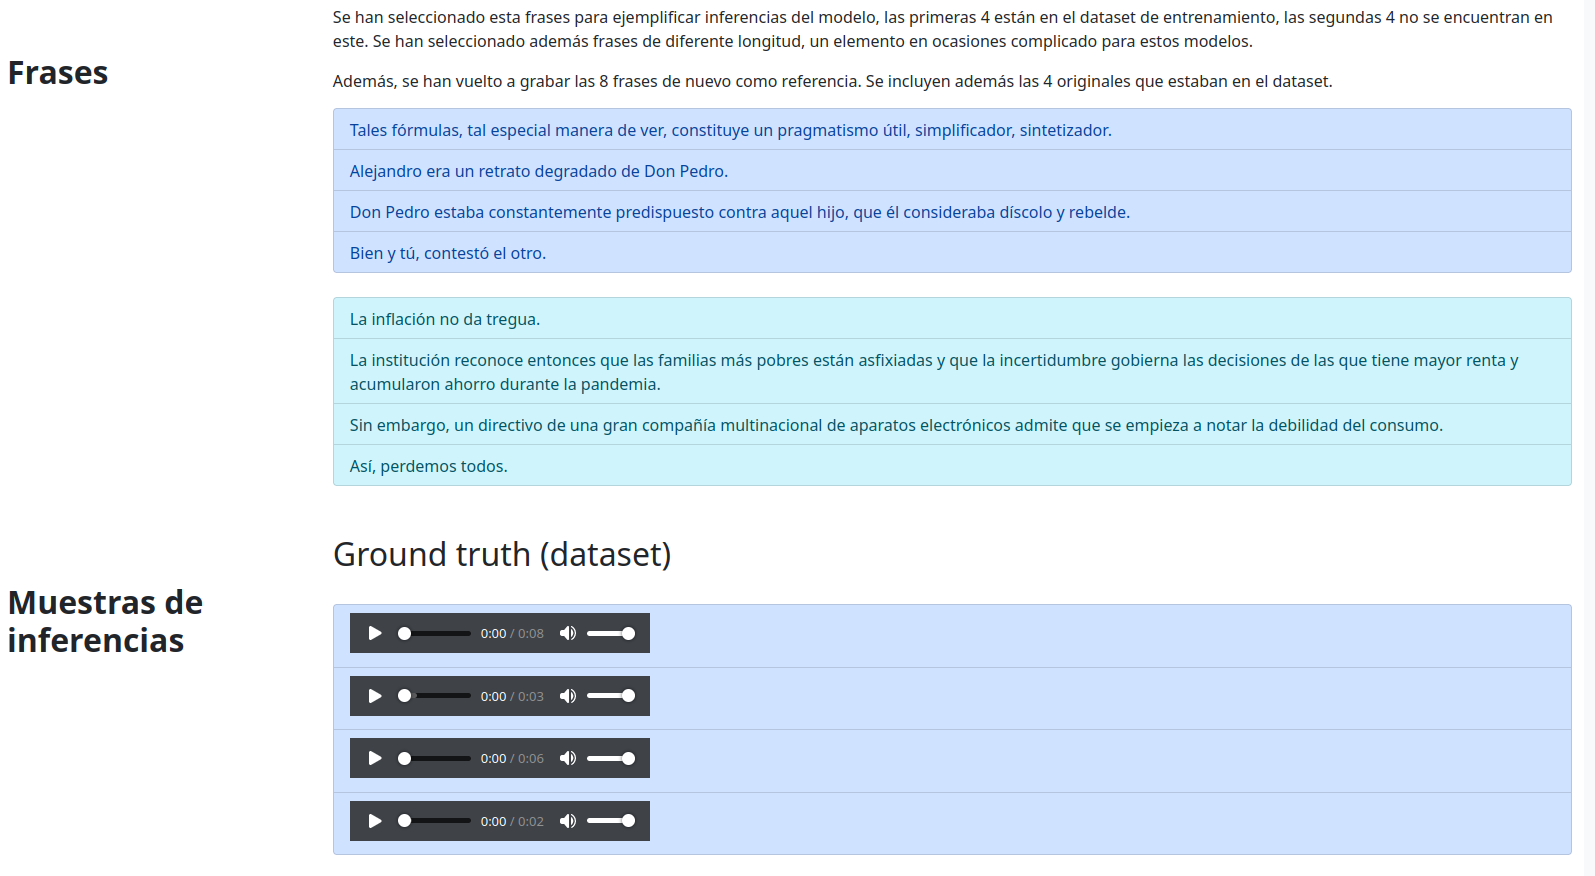
\includegraphics[width=14cm]{8_entregables_img/infer-sample-0.png}
\caption{Web con inferencias precalculadas a modo de ejemplo y comparativa.}
\label{fig:figure1}
\end{figure}


La web está disponible aquí como una simple GitHub Page: \url{https://daniel-dona.github.io/tfg-inference-samples/}


\subsection{Interfaz de pruebas}

Se han preparado varias interfaces con las que mostrar los resultados de los modelos entrenados así como permitir interactuar con ellos según se desee.

\subsubsection{Bot en Telegram}

Se trata de un usuario especial en la aplicación de chat Telegram que responde al comando /tts [texto] devolviendo una nota de voz con el resultado de la inferencia del modelo. Esta interfaz se pensó originalmente como demostración no solo de los resultados sino además de la generación en tiempo real de dichos resultados.


\begin{figure}[h]
\centering
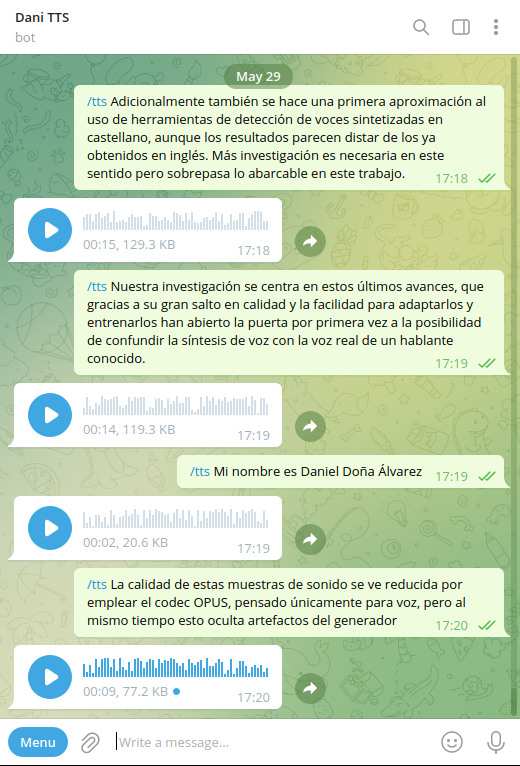
\includegraphics[width=8cm]{8_entregables_img/telegram_0.png}
\caption{Aspecto de la comunicación con el bot desplegado.}
\label{fig:figure1}
\end{figure}


Se puede interactuar con esta interfaz accediendo a esta dirección: \url{https://t.me/dani_tts_bot}

\subsubsection{Demo en HuggingFace Spaces}

HuggingFace es un ecosistema pensado para compartir datasets, modelos entrenados y demostraciones de estos modelos entre la comunidad de Aprendizaje Computacional.

Hemos desplegado una demostración del modelo también allí, estando disponible tanto su código como una interfaz sencilla para realizar inferencias.

\begin{figure}[H]
\centering
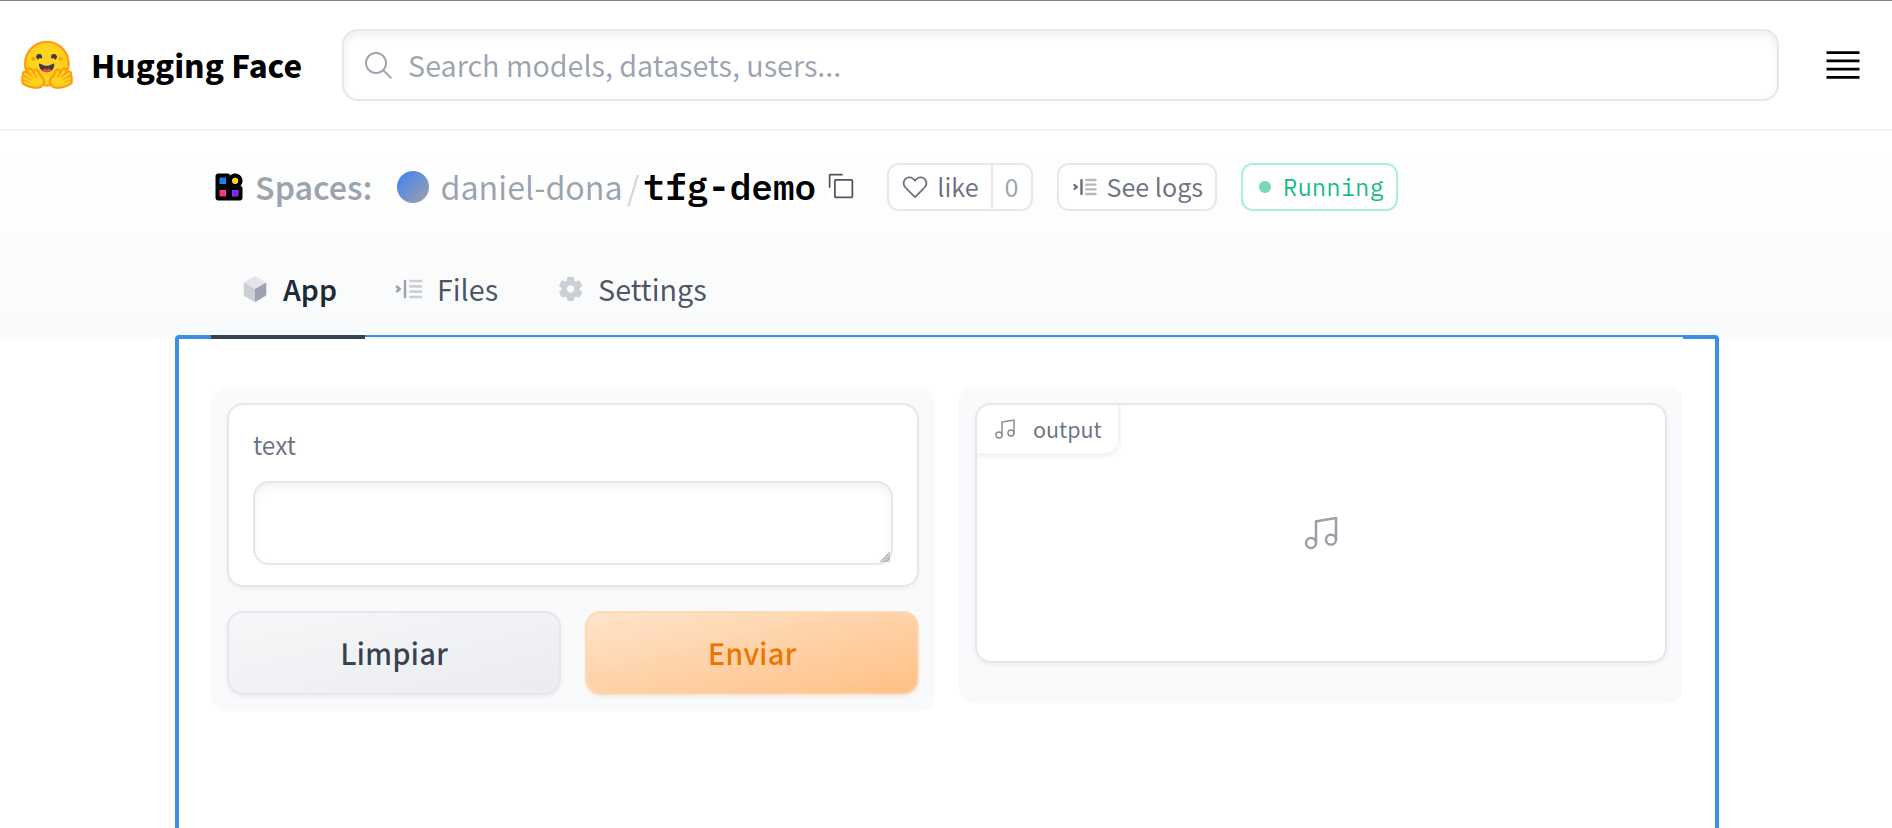
\includegraphics[width=14cm]{8_entregables_img/entrega_hf_0.png}
\caption{Interfaz de pruebas en la plataforma de HuggingFace.}
\label{fig:figure1}
\end{figure}

Se puede consultar en esta dirección: \url{https://huggingface.co/spaces/daniel-dona/tfg-demo}

\newpage 
\newpage \section{Glosario}

\begin{itemize}
    
\item IA: Acrónimo de Inteligencia artificial, disciplina que intenta imitar o emular comportamientos o procesos que se consideran inteligentes. 

\item Aprendizaje Computacional: rama que estudia mecanismos que permitan a un sistema mejorar a partir de la experiencia. Habitualmente se suele relacionar con la resolución de problemas planteados en el ámbito de la Inteligencia Artificial.

\item TTS: Acrónimo del inglés "text to speech", método de síntesis de voz mediante una entrada de texto.

\item Deepfake: Acrónimo del inglés "deep learning fake", falsificación generada total o parcialmente mediante el uso de modelos de inteligencia artificial.

\item Entrenar (modelos): Proceso por el cual un modelo de Aprendizaje Computacional extrae características o información relevante de un conjunto de datos para adquirir alguna capacidad funcional relacionada con dichos datos.

\item Fonema: Unidad sonora mínima articulable en una palabra, el proceso del habla humana.

\item Toolkit: Del inglés "conjunto de herramientas", habitualmente una recolección de distintos componentes de software o herramientas que se usan de forma conjunta o que su uso pertenece a un mismo dominio, facilitando así el cumplimiento de ciertas tareas en un mismo ecosistema.

\item Notebook (Google Colab, Jupyter, etc...): Tipo de fichero especial que contiene una mezcla de código y explicaciones, habitualmente empleados en contextos de docencia y en demostraciones guiadas para exponer el funcionamiento de una pieza de software.

\item Código abierto: forma de licencia para la publicación del código fuente de un producto de software que se caracteriza por dar especial libertad al usuario para su examen, modificación o uso en nuevas creaciones.

\item Dataset: Conjunto de datos especialmente pensado y preparado para su procesamiento de forma automatizada y para fines diversos. 



\end{itemize}
\newpage 

\listoffigures

\newpage 
\newpage \section{Bibliografía}

\begin{enumerate}

% Resumen e introducción

\label{RI_1}
\item{DUTOIT, Thierry. \emph{An Introduction to Text-to-Speech Synthesis. Text, Speech and Language Technology}. Disponible en: \url{https://doi.org/10.1007/978-94-011-5730-8}}

\label{RI_2}
\item{Revista FORBES. \emph{Fraudsters Cloned Company Director’s Voice In \$35 Million Bank Heist, Police Find}. Disponible en: \url{https://www.forbes.com/sites/thomasbrewster/2021/10/14/huge-bank-fraud-uses-deep-fake-voice-tech-to-steal-millions/}}

\label{RI_3}
\item{Revista HD-TECNOLOGÍA. \emph{Un programa de Deepfake para la voz se usó para robar U\$S 243.000}. Disponible en: \href{https://www.hd-tecnologia.com/un-programa-de-deepfake-para-la-voz-se-uso-para-robar-us-243-000/}{https://www.hd-tecnologia.com/un-programa-de-deepfake-para-la-voz-se-uso-para-robar-us-243-000/}}


\label{RI_4}
\item{INE, publicación web \emph{Población que usa Internet (en los últimos tres meses).} \url{https://www.ine.es/ss/Satellite?L=es_ES&c=INESeccion_C&cid=1259925528782&p=1254735110672&pagename=ProductosYServicios\%2FPYSLayout}}

% Estado del Arte

\label{EA_1}
\item{Repositorio de MBROLA. Disponible en: \url{https://github.com/numediart/MBROLA/}}


\label{EA_4}
\item{ARIK, Sercan O et. al. \emph{Deep Voice: Real-time Neural Text-to-Speech}. Disponible en: \url{https://arxiv.org/abs/1702.07825}}

\label{EA_5}
\item{WANG, Yuxuan et. al. \emph{Tacotron: Towards End-to-End Speech Synthesis}. Disponible en: \url{https://arxiv.org/abs/1703.10135}}

\label{EA_6}
\item{SHEN, Jonathan et. al \emph{Natural TTS Synthesis by Conditioning WaveNet on Mel Spectrogram Predictions}. Disponible en: \url{https://arxiv.org/abs/1712.05884}}

\label{EA_7}
\item{OORD, Aaron van den et. al \emph{WaveNet: A Generative Model for Raw Audio}. Disponible en: \url{https://arxiv.org/abs/1609.03499}}

\label{EA_8}
\item{KIM, Jaehyeon et. al \emph{Conditional Variational Autoencoder with Adversarial Learning for End-to-End Text-to-Speech}. Disponible en: \url{https://arxiv.org/abs/2106.06103}}

\label{EA_9}
\item{CASANOVA, Edresson et. al \emph{YourTTS: Towards Zero-Shot Multi-Speaker TTS and Zero-Shot Voice Conversion for everyone}. Disponible en: \url{https://arxiv.org/abs/2112.02418}}

\label{EA_2}
\item{Repositorio de ESPnet. Disponible en: \url{https://github.com/espnet/espnet}}

\label{EA_3}
\item{Repositorio de Coqui-AI TTS. Disponible en: \url{https://github.com/coqui-ai/TTS}}


% Resultados
\label{RES_1}
\item{VASWANI, Ashish et. al \emph{Attention Is All You Need}. Disponible en: \url{https://arxiv.org/abs/1706.03762}}


\label{RES_1_1}
\item{KIM, Jaehyeon et. al \emph{Glow-TTS: A Generative Flow for Text-to-Speech via Monotonic Alignment Search}. Disponible en: \url{https://arxiv.org/abs/2005.11129}}


\label{RES_2}
\item{DIRAC, Leo. \emph{Conferencia en el Seattle Applied Deep Learning}. 2020. Disponible en: \url{https://www.youtube.com/watch?v=S27pHKBEp30}}

\label{RES_3}
\item{Recomendación \emph{P.800.1} del ITU. Disponible en: 
\url{https://www.itu.int/rec/T-REC-P.800.1-201607-I/en}}

\label{RES_4}
\item{Wiki del proyecto Mozilla TTS. Disponible en: \url{https://github.com/mozilla/TTS/wiki/Dataset\#what-makes-a-good-dataset}}

\label{RES_5}
\item{Repositorio de la implementación de Tacotron 2 realizada por NVIDIA. Disponible en: \url{https://github.com/NVIDIA/tacotron2}}

\label{RES_6}
\item{Descripción de la web \emph{fakeyou.com}. Disponible en: \url{https://github.com/jaywalnut310/vits}}

\label{RES_7}
\item{Repositorio de la implementación original de VITS. Disponible en: \url{https://fakeyou.com/about}}


% Discusión

% Conclusiones

\label{CON_1}
\item{ASVspoof 2021 Workshop. Disponible en: \url{https://www.asvspoof.org/workshop}}


% Anexos

\label{AX_1}
\item{Dataset LJSpeech, consultable en \url{https://keithito.com/LJ-Speech-Dataset/}}


\end{enumerate}
\newpage 
\newpage \section{Anexos}

En las siguientes páginas se han redactado algunos análisis, informaciones o datos que no se consideraban relevantes detallar en el hilo vertebrador del trabajo pero que aún así se considera que merece la pena incluirlos en el trabajo.


\newpage 
\subsection{Grabación de datasets}
\label{Grabación de datasets}

Una de las primeras tareas que se identificaron como esenciales para este proyecto fue la obtención de algún conjunto de datos de voz de referencia con el que realizar experimentos de entrenamiento.

Aunque existen varios relativamente conocidos en castellano, muchos derivados de proyectos como LibriVox\footnote{Sitio web dedicado a compartir audiolibros que han sido grabados de forma colaborativa.}, su calidad no es la adecuada y no son sistemáticos como para obtener los mejores resultados posibles y en el menor tiempo posible. 

Los datasets que se suelen emplear para los entrenamientos en inglés por otra parte suelen constar de decenas de horas de audio en decenas de miles de clips, algo que escapa a las posibilidades materiales y humanas de este trabajo.

Se decidió optar por una solución intermedia, que cuidase la calidad del sonido lo máximo posible para compensar lo modesto del número de muestras.

\subsubsection{Hardware}

Aunque cualquier micrófono moderno es capaz de capturar con suficiente claridad la voz humana para propósitos comunicativos, no todos los micrófonos son capaces de capturarla con el mismo grado de fidelidad.

Existen numerosos parámetros que miden las características técnicas de un micrófono y lo adecuado o no para un fin particular. En nuestra situación es bastante importante reducir la relación señal/ruido sin perder calidad.

El micrófono empleado para la grabación de las muestras ha sido un Rode NT USB que permite una conversión A/D de 16 bits a 48kHz\footnote{Estrictamente, considerando el rango de audición humana 20Hz - 20kHz según el Teorema de muestreo de Shannon no necesitaríamos más de 40kHz para reproducir de forma íntegra una señal de dicho ancho de banda. Pero experimentalmente se sabe que aumentar dicha frecuencia de muestreo algo más reduce los efectos negativos que puede tener la conversión analógico-digital.}.

Este micrófono tiene un patrón polar cardioide, lo que significa que la mayoría de la señal procederá del sonido que tenga delante, atenuando notablemente la parte posterior y parcialmente los laterales.

Este es un primer paso para gestionar de forma adecuada el ruido ambiental ya que no se dispone de condiciones de estudio para la grabación sino de un entorno doméstico y urbano.

\begin{figure}[H]
\centering
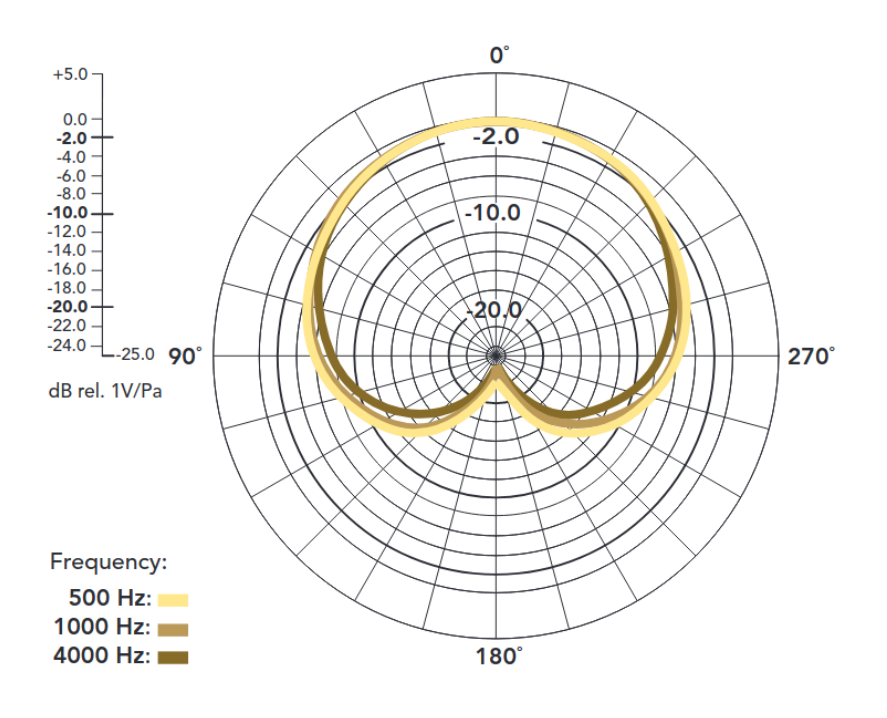
\includegraphics[width=14cm]{Z_anexos_img/rode-nt-polar.png}
\caption{Diagrama polar de la respuesta espacial.}
\label{fig:figure1}
\end{figure}


La respuesta de frecuencias del micrófono por otra parte es mayormente plana, lo que es algo positivo si esperamos una reproducción fiel de la señal original una vez digitalizada.

\begin{figure}[H]
\centering
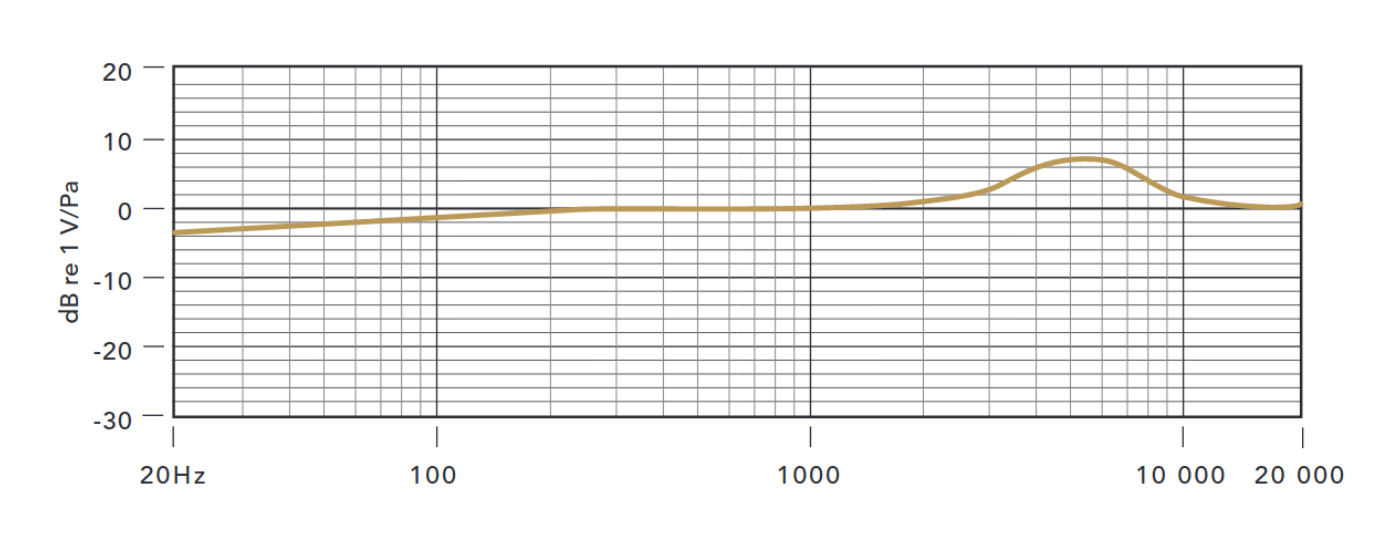
\includegraphics[width=14cm]{Z_anexos_img/rode-nt-response.png}
\caption{Diagrama de respuesta de frecuencias.}
\label{fig:figure1}
\end{figure}

\subsubsection{Software}

No se identificó ningún software específico para la grabación y gestión de datasets de audio, por lo menos no que fuese adecuado para la simple grabación de clips a partir de textos de partida. Se decidió implementar una aplicación simple que tomase una entrada de texto, la segmentase en frases y las presentase al hablante para su grabación de la forma más sencilla posible.

La interfaz es la habitual en una consola de comandos, puesto que era una herramienta para uso exclusivo de la investigación y no sería un producto final para otros usuarios no se consideró ofrecer una interfaz mejor.

\begin{figure}[H]
\centering
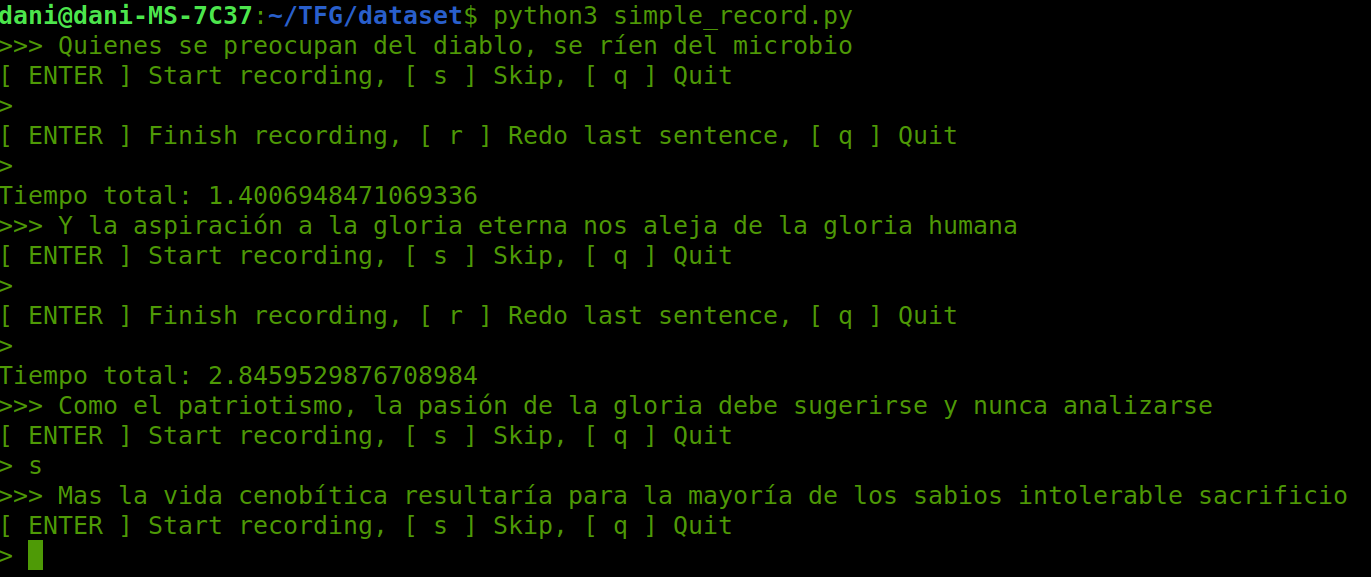
\includegraphics[width=14cm]{Z_anexos_img/record-0.png}
\caption{Interfaz de consola con la que se generó el dataset de audio.}
\label{fig:figure1}
\end{figure}

El funcionamiento es muy simple, cada frase a grabar se muestra por pantalla, el inicio de la grabación comienza cuando se pulsa ENTER y finaliza igualmente cuando se pulsa ENTER. Si ha habido algún error de grabación se puede repetir la última frase grabada y si el texto por el motivo que sea se considera inadecuado para el dataset se puede saltar a la siguiente frase.

Por ejemplo, para el caso base que queremos entrenar se han ignorado nombres propios y términos que no siguen las reglas propias de pronunciación del castellano. Excluimos esencialmente extranjerismos. 

El programa graba cada fragmento como un fichero .wav separado, bien con la calidad original de grabación o bien con algún procesamiento o modificación. Al mismo tiempo se registra en un fichero una nueva entrada que contiene la ruta al fichero de audio y el fragmento de texto.

Este será el formato del dataset final, se ha empleado una barra vertical para separar los campos del fichero porque es el formato original del dataset LJSpeech y es más rápido adaptar modelos ya existentes.

\subsubsection{Reducción de ruido}

Por mucho que se intentó encontrar el ambiente más apartado de ventanas y otros sonidos ambientales fue imposible eliminar del todo el ruido de las muestras simplemente grabadas. 

Para postprocesar los ficheros de sonido y reducir aún más la cantidad de ruido base en el dataset se probaron diferentes herramientas de edición de sonido.

Audacity es un programa de edición de audio bastante conocido y es software libre, entre las diferentes herramientas de manipulación de sonido que tiene se encuentra un reductor de ruido\footnote{Más información en \url{https://manual.audacityteam.org/man/noise_reduction.html}}. Su funcionamiento consiste en seleccionar una muestra que contenga únicamente ruido, de donde el programa extraerá las frecuencias que deberá reducir en el resto de la señal.

Esta forma de reducir el ruido funciona bien cuando el ruido es constante, pero no en el caso de ruidos que puedan variar en el tiempo ni especialmente puntuales\footnote{Su propia documentación así lo indica: «It is not suitable for individual clicks and pops, or irregular background noise such as from traffic or an audience»}.

La segunda opción que se barajó fue emplear un filtro del proyecto Xiph denominado RNNoise\footnote{\url{https://github.com/xiph/rnnoise}}, que ha sido entrenado con muestras reales de ruido y para el que tenemos modelos\footnote{\url{https://github.com/GregorR/rnnoise-models}} específicamente entrenados para el procesamiento de voz.

Esta fue la forma en la que finalmente se procesaron todas las muestras de audio por demostrar ofrecer los mejores resultados frente a las diferentes fuentes de ruido.

[Ejemplo de uso con ffmpeg]

\newpage 
\subsection{Entrenamiento en Google Colab}
\label{Entrenamiento en Google Colab}

Aunque la mayor parte de los entrenamientos se han realizado en local empleando hardware propio, en cierto momento se consideró que podía ser adecuado realizar más de un entrenamiento de manera simultánea.

El precio actual de las GPUs volvía esto imposible si se quería seguir trabajando simplemente en local, por lo que se exploraron las diferentes opciones posibles y su coste.

Google Colab es ahora mismo la opción más económica para el entrenamiento de modelos que requieran del uso intensivo de GPU. Existen dos rangos de precios: en el primer caso por 10€ se accede a una cuenta Colab Pro, en el segundo caso por 50€ al mes se obtiene una cuenta Colab Pro +.

Google es intencionalmente poco preciso sobre los derechos y recursos a los que se puede acceder en ambos casos, pero la experiencia de los usuarios indica que los recursos de hardware no están asegurados y simplemente se reparten entre los usuarios. Este reparto es una cola con prioridades donde los usuarios Pro + tiene preferencia.

Google Colab esencialmente proporciona acceso a GPUs Nvidia P100 (PCIe) y aceleradores Nvidia T4, en nuestro caso suficiente para los entrenamientos pero algo más lento que el entrenamiento en local.

\begin{figure}[H]
\centering
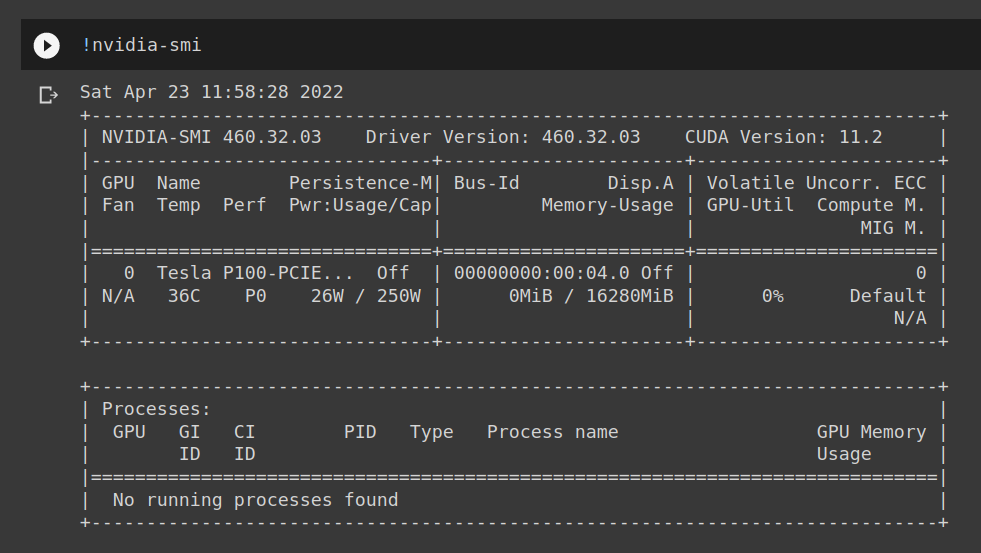
\includegraphics[width=14cm]{Z_anexos_img/colab-1.png}
\caption{Ejemplo de GPU asignada a una instancia de Google Colab Pro +.}
\label{fig:figure1}
\end{figure}

El problema esencial de Google Colab es que su diseño no está orientado al funcionamiento en sesiones largas, sea cual sea el tipo de cuenta que uno tenga. En el caso de cuentas Pro + se asegura un máximo de 24h de duración de las sesiones, en las cuentas Pro y gratuitas es notablemente menor.

Para poder sortear este problema se elaboraron una serie de herramientas que permitían reanudar el entrenamiento tras el fin de la sesión de forma rápida y conservando en todo momento el progreso del entrenamiento. Los notebooks de Colab se ejecutan en un entorno virtualizado que se elimina una vez finaliza la sesión por lo que todos los datos se pierden de otra forma.

Un ejemplo de notebook de Colab empleado se puede consultar aquí: \url{https://colab.research.google.com/drive/1ph_y84bRc-hKtFhmI4tDAiOZpm-LQuUn}

El conjunto de scripts empleados para entrenar, subir los resultados parciales a una instancia de NextCloud y reanudar los entrenamientos se encuentran en este repositorio: \url{https://github.com/daniel-dona/TFG-colab-train-helpers}

De forma resumida, el funcionamiento del notebook es el siguiente:

\begin{enumerate}
    \item Descarga de datasets y herramientas
    \item Descarga del último checkpoint guardado
    \item Inicio o continuación del entrenamiento
    \item Lanzamiento en segundo plano de un proceso que suba el último checkpoint a un almacenamiento remoto
\end{enumerate}

Este mecanismo se empleó para entrenar varios modelos con el dataset LJSpeech, especialmente las primeras pruebas con el modelo VITS.

\newpage 
\subsection{Análisis de datasets}
\label{Análisis de datasets}

Prácticamente la totalidad de modelos estudiados usan el dataset LJSpeech \hyperref[AX_1]{[23]} como referencia. Este modelo grabado a partir de una única hablante se caracteriza por su alta calidad y su tono neutro.

El dataset contiene un total de 13100 clips de audio, con un total de 225715 palabras. Contiene aproximadamente 24 horas de grabación en total y los clips de sonido oscilan entre los 2 segundos y los 10 segundos.

Para nuestras pruebas nos interesaba especialmente estudiar no tanto el dataset propiamente sino el resultado de convertirlo a fonemas con algunas de las herramientas (entrenadas o paramétricas) que nuestro toolkit incluía. 

Aunque es posible entrenar los modelos directamente a partir de caracteres y dejar que los mecanismos de atención del modelo encuentren las diferencias fonéticas del lenguaje a partir de los caracteres anteriores y siguientes, se suelen emplear conversores a fonemas en la mayoría de modelos por hacer más rápido el aprendizaje.

En primer lugar analizamos la presencia estadística de los fonemas empleando un histograma:

\begin{figure}[H]
\centering
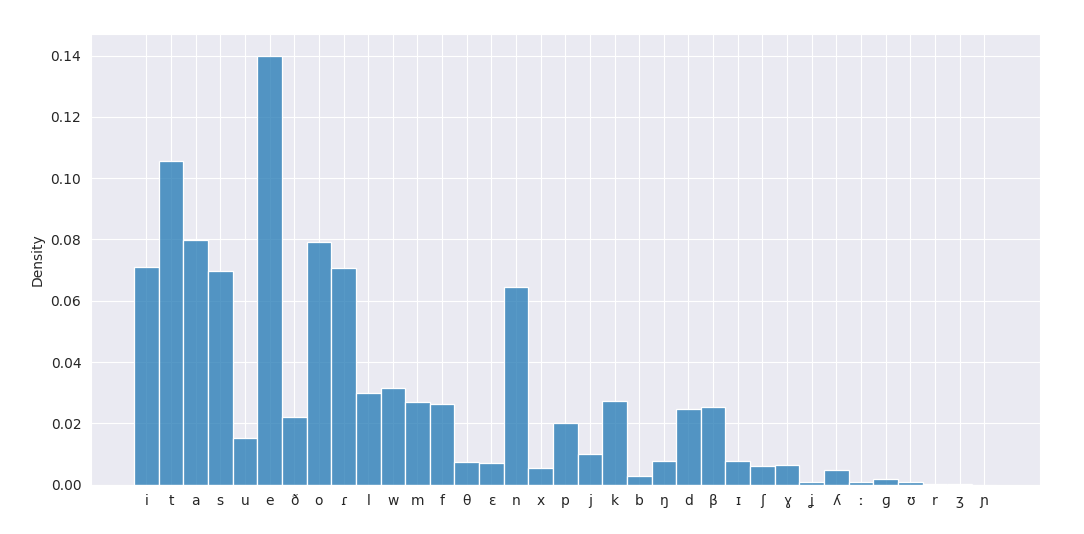
\includegraphics[width=14cm]{Z_anexos_img/ljs-1.png}
\caption{Histogramas de fonemas en LJSpeech}
\label{fig:figure1}
\end{figure}

Aunque ciertos fonemas se encuentran claramente infrarepresentados en el dataset, el tamaño del propio dataset nos permite ignorar esto. 

Sabíamos que algunos modelos paramétricos empleaban no fonemas, sino parejas de fonemas para representar la unidad básica para la síntesis de voz. Por ello decidimos además analizar la presencia de ciertas parejas de fonemas.

\begin{figure}[H]
\centering
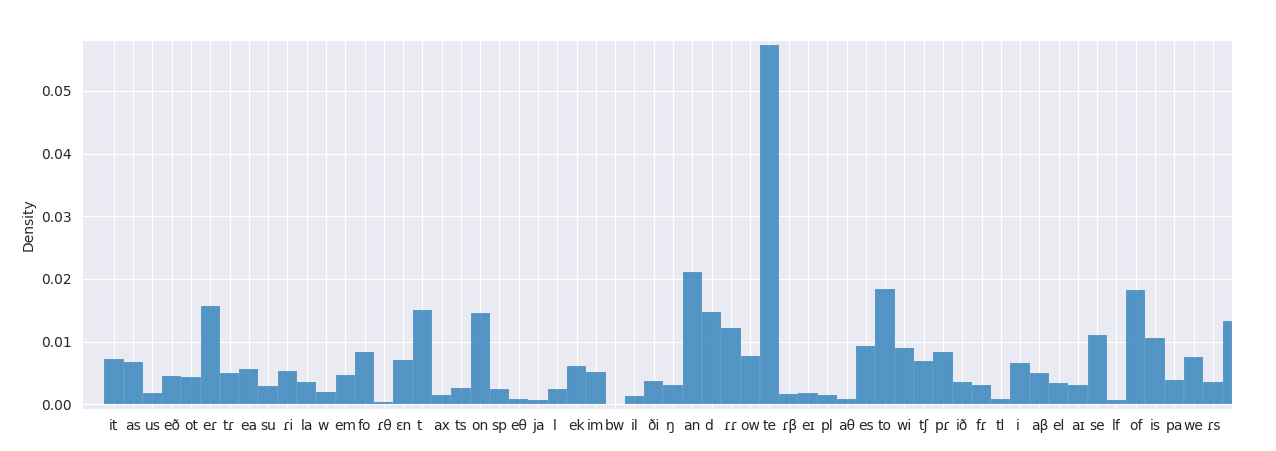
\includegraphics[width=14cm]{Z_anexos_img/ljs-2.png}
\caption{Histogramas de pares de fonemas en LJSpeech (más frecuentes).}
\label{fig:figure1}
\end{figure}

\begin{figure}[H]
\centering
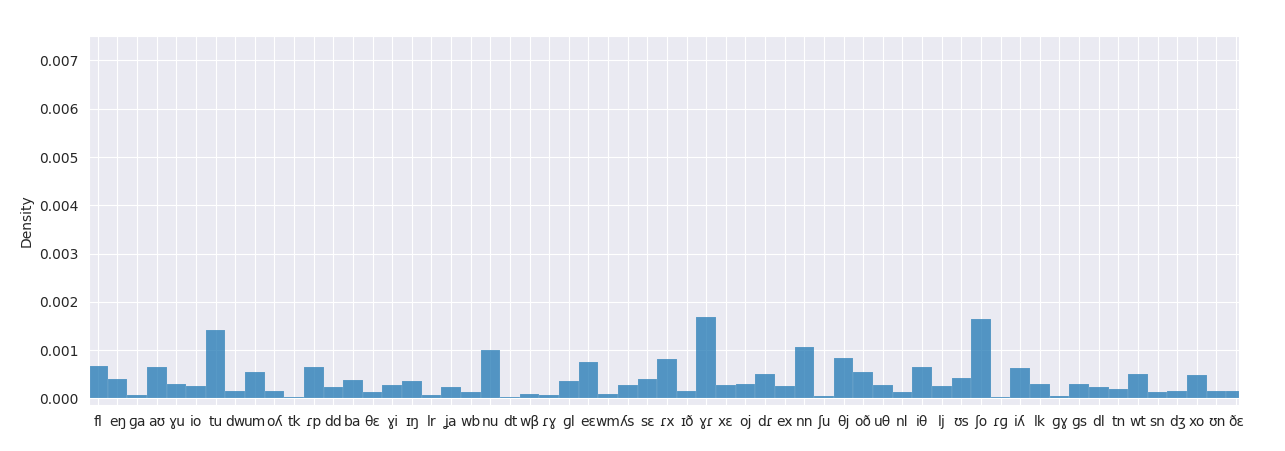
\includegraphics[width=14cm]{Z_anexos_img/ljs-3.png}
\caption{Histogramas de pares de fonemas en LJSpeech (menos frecuentes).}
\label{fig:figure1}
\end{figure}



En este caso encontramos que ciertas parejas de fonemas aparecen de forma muy muy escasa en el dataset. De la misma forma que ciertos grafemas son mucho más comunes que otros en una lengua, es esperable que ciertos fonemas y parejas de fonemas sean raros igualmente.

Sabemos que este dataset es el más empleado por ofrecer unos buenos resultados en inglés, por lo que podemos asumir que la inmensa mayoría de combinaciones fonéticas están cubiertas. 

Sabiendo que nosotros no podemos aspirar a un dataset tan grande, esta distribución de los datos puede suponer que con un dataset pequeño ciertas palabras se sinteticen con notablemente peor calidad que otras o que directamente el modelo no haya sido entrenado con un fonema que aparezca en una inferencia determinada.

Esto último también puede suceder si se intenta inferir a partir de un texto/fonemas de un idioma distinto o una variedad dialectal distinta.

\newpage 
\subsection{Entorno de entrenamiento}
\label{Entorno de entrenamiento}

Con anterioridad se han comentado las dificultades para realizar entrenamientos largos empleando Google Colab, es por ello que se relegó a un segundo plano como entorno para realizar este tipo de tareas. El entorno principal para el entrenamiento fue en su lugar un computador propio con la siguiente configuración de hardware:

\begin{itemize}
    \item CPU: AMD Ryzen 9 5900X (12 cores/24 threads)
    \item Main memory: DDR4 3600 CL18 (32 GB)
    \item GPU: Nvidia RTX3080 Ti (12 GB), 10240 CUDA cores
    \item Disco: NVMe WD 1TB SN500 
\end{itemize}

El sistema operativo base en el que se han desarrollado los entrenamientos es Ubuntu 20.04, siendo la versión de Python 3 propia de la distribución la 3.8.10.

Los drivers de NVIDIA que habilitaron poder emplear aceleración mediante CUDA fueron los 510.47.03. 

NVIDIA emplea un concepto denominado Compute Capability para identificar características entre las diferentes generaciones de aceleradores y tarjetas gráficas. La versión de esta tarjeta gráfica es la 8.6, también identificada en algunas librerías como SM\_86.

Además los drivers de NVIDIA específicamente para CUDA tienen diferentes versiones, siendo los más recientes la versión CUDA 11.6. Esta versión, junto a la Compute Capability tiene que ser compatible con las diferentes librerías que quieran hacer uso de la GPU para acelerar cálculos.

En el caso de Torch, la librería principal para los entrenamientos, se tuvo que instalar una versión específica para poder hacer uso de los recursos de computación disponibles.

\begin{lstlisting}
python3 -m pip install torch==1.10.2+cu113 torchvision==0.11.3+cu113 torchaudio==0.10.2+cu113 -f https://download.pytorch.org/whl/cu113/torch_stable.html
\end{lstlisting}

Durante los entrenamientos el uso de la tarjeta gráfica supone un consumo de energía de aproximadamente 300W adicionales al consumo del resto del sistema, esto supone una gran cantidad de calor que puede ser problemático para la vida útil de los componentes electrónicos.

\begin{figure}[H]
\centering
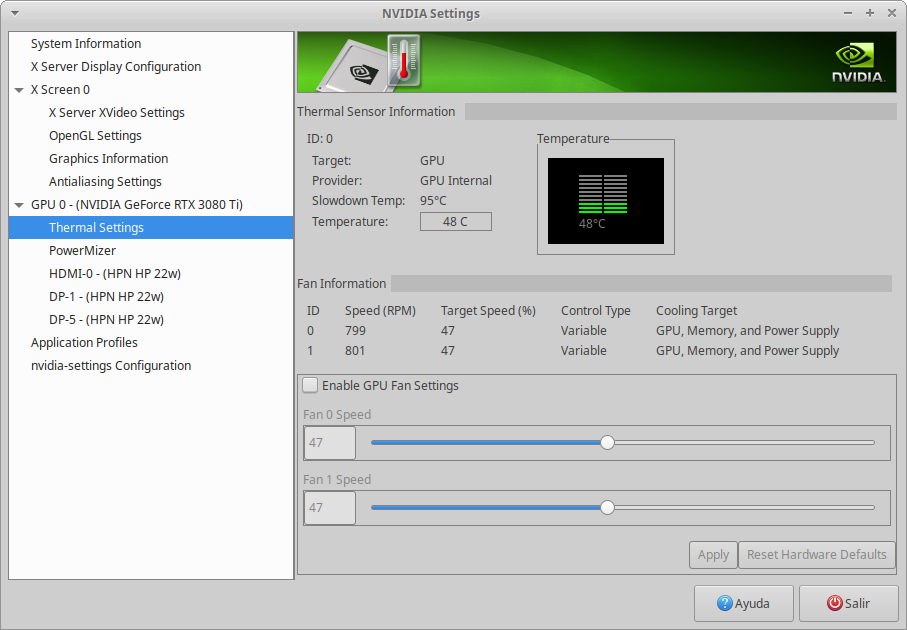
\includegraphics[width=14cm]{Z_anexos_img/nvidia-smi.png}
\caption{Interfaz de gestión de NVIDIA en Linux.}
\label{fig:figure1}
\end{figure}

Para mantener el hardware en una zona segura, se ha forzado manualmente el uso intensivo de los ventiladores de la tarjeta gráfica para bajar lo máximo posible la temperatura. Esto en algunos momentos ha sido conflictivo con las labores de grabación del dataset de voz al generar bastante ruido.

\end{document}

